% !TeX encoding = UTF-8
\chapterimage{chap34.jpg}
\chapter{August}
\section{Week \Rmnum{1}}
\textcolor{orange}{August 1}

1. 已知$f(x)$为奇函数,则$f_{+}'(0)$存在和$f(x)$在$x=0$处可导关系
\myspace{1}
\begin{solution}
	
	(1). 充分性
	
	$$\lim\limits_{x\to 0^{+}}\dfrac{f(x)-f(0)}{x}=A\Rightarrow \lim\limits_{x\to 0^{+}}f(x)=0$$
	
	我们可以得到: 
	$$\lim\limits_{x\to 0^{-}}\dfrac{f(x)-f(0)}{x}=\lim\limits_{x\to 0^{+}}\dfrac{f(-x)-f(0)}{-x}=\lim\limits_{x\to 0^{+}}\dfrac{-f(x)-f(0)}{-x}=A$$
	
	我们得到: $$\lim\limits_{x\to 0^{+}}\dfrac{f(x)-f(0)}{x}=\lim\limits_{x\to 0^{-}}\dfrac{f(x)-f(0)}{x}=A$$
	
	充分性成立
	
	(2). 必要性
	
	$$f(x)\text{在}x=0\text{处可导}\Rightarrow \lim\limits_{x\to 0^{+}}\dfrac{f(x)-f(0)}{x}=\lim\limits_{x\to 0^{-}}\dfrac{f(x)-f(0)}{x}=A$$
	
	必要性成立
	
	综上所述,$f_{+}'(0)$存在是$f(x)$在$x=0$处可导的充要条件.
\end{solution} 
\myspace{1}

2. 求$\int_{0}^{1}dx\int_{1-x}^{2-x}e^{(x+y)^2}(\sin^2x+\cos^2y)dy+\int_{1}^{2}dx\int_{0}^{2-x}e^{(x+y)^2}(\sin^2x+\cos^2y)dy$
\myspace{1}
\begin{solution}
	
	我们画出二重积分的积分区域,不难发现积分区域关于直线$y=x$对称,原二重积分等价于: 
	$$I=\int_{0}^{1}dx\int_{1-x}^{2-x}e^{(y+x)^2}(\sin^2y+\cos^2x)dy+\int_{1}^{2}dx\int_{0}^{2-x}e^{(y+x)^2}(\sin^2y+\cos^2x)dy$$
	
	我们得到: 
	\begin{eqnarray*}
		2I&=&\int_{0}^{1}dx\int_{1-x}^{2-x}2e^{(x+y)^2}dy+\int_{1}^{2}dx\int_{0}^{2-x}2e^{(x+y)^2}dy\\
		&=&\int_{0}^{\frac{\pi}{2}}d\theta\int_{\frac{1}{\sin\theta+\cos\theta}}^{\frac{2}{\sin\theta+\cos\theta}}2re^{r^2(1+\sin 2\theta)}dr\\
		&=&\int_{0}^{\frac{\pi}{2}}\dfrac{e^4-e}{1+\sin2\theta}d\theta\\
		I&=&\dfrac{e^4-e}{2}\int_{0}^{\frac{\pi}{2}}\dfrac{\frac{1}{\cos^2\theta}}{(1+\tan\theta)^2}d\theta\\
		&=&\dfrac{e^4-e}{2}\int_{0}^{+\infty}\dfrac{1}{(1+x)^2}dx\\
		&=&\dfrac{e^4-4}{2}
	\end{eqnarray*}
\end{solution}
\myspace{1}

\textcolor{orange}{August 2}

1. 已知函数$f(x)$在$x=x_{0}$的邻域内可导,则$f'(x_{0})>0$是$f(x)$在$x=x_{0}$的某邻域内单调递增之间关系
\myspace{1}
\begin{solution}
	
	(1). 充分性
	$$\lim\limits_{x\to x_{0}}\dfrac{f(x)-f(x_{0})}{x-x_{0}}=A>0$$
	
	我们可以得出,$x\in(x_{0}-\delta,x_{0}),f(x)<f(x_{0})$;$x\in(x_{0},x_{0}+\delta),f(x)>f(x_{0})$,并不能得出函数的单调性.
	
	(2). 必要性
	
	$f(x)$在某邻域内单调递增,我们只能得出$f'(x_{0})\geq 0$
	
	综上所述,$f'(x_{0})>0$是$f(x)$在$x=x_{0}$的某邻域内单调递增的既不充分也不必要条件.
\end{solution}
\myspace{1}

2. $I_{n}=\int_{1}^{+\infty}\dfrac{\sqrt{t-1}}{t^n}dt\ (n\geq 2)$,求$\lim\limits_{n\to+\infty}\dfrac{I_{n+1}}{I_{n}}$
\myspace{1}
\begin{solution}
	
	我们令$t=\dfrac{1}{\cos^2 x},\ x\in(0,\dfrac{\pi}{2}),\ dt=\dfrac{2\sin x}{\cos^3 x}$,我们可以得到: 
	\begin{eqnarray*}
		I_{n}&=&\int_{0}^{\frac{\pi}{2}}\dfrac{\sin x}{\cos x}\cos^{2n}x\dfrac{2\sin x}{\cos^3 x}dx\\
		&=&2\int_{0}^{\frac{\pi}{2}}\cos^{2n-4}xdx-2\int_{0}^{\frac{\pi}{2}}\cos^{2n-2}xdx
	\end{eqnarray*}
	由此我们可以得到: 
	$$\left\lbrace
	\begin{array}{l}
		I_{n+1}=2\int_{0}^{\frac{\pi}{2}}\cos^{2n-2}xdx-2\int_{0}^{\frac{\pi}{2}}\cos^{2n}xdx\\
		I_{n}=2\int_{0}^{\frac{\pi}{2}}\cos^{2n-4}xdx-2\int_{0}^{\frac{\pi}{2}}\cos^{2n-2}xdx
	\end{array}
	\right. $$
	
	我们得到: 
	$$\dfrac{I_{n+1}}{I_{n}}=\dfrac{\int_{0}^{\frac{\pi}{2}}\cos^{2n-2}xdx-\int_{0}^{\frac{\pi}{2}}\cos^{2n}xdx}{\int_{0}^{\frac{\pi}{2}}\cos^{2n-4}xdx-\int_{0}^{\frac{\pi}{2}}\cos^{2n-2}xdx}$$
	
	我们计算: 
	\begin{eqnarray*}
		J_{2n}&=&\int_{0}^{\frac{\pi}{2}}\cos^{2n}xdx\\
		&=&\int_{0}^{\frac{\pi}{2}}\cos^{2n-1}xd\sin x\\
		&=&(2n-1)\int_{0}^{\frac{\pi}{2}}\sin^{2} x\cos^{2n-2}xdx\\
		&=&(2n-1)\int_{0}^{\frac{\pi}{2}}\cos^{2n-2}xdx-(2n-1)\int_{0}^{\frac{\pi}{2}}\cos^{2n}xdx\\
		&=&(2n-1)J_{2n-2}-(2n-1)J_{2n}\\
		J_{2n}&=&\dfrac{2n-2}{2n}J_{2n-2}
	\end{eqnarray*}

	我们得到: 
	$$\dfrac{I_{n+1}}{I_{n}}=\dfrac{J_{2n-2}-J_{2n}}{J_{2n-4}-J_{2n-2}}=\dfrac{\frac{2}{2n}J_{2n-2}}{\frac{2}{2n-2}J_{2n-4}}=\dfrac{n-1}{n}\dfrac{2n-4}{2n-2}=\dfrac{n-2}{n}$$
	
	$$\lim\limits_{n\to+\infty}\dfrac{I_{n+1}}{I_{n}}=\lim\limits_{n\to+\infty}\dfrac{n-2}{n}=1$$
\end{solution}
\myspace{1}

\textcolor{orange}{August 3}

1. 设函数$f(x)$在$x=x_{0}$的某个邻域内有定义,下列命题中正确的个数:  
\begin{itemize}
	\item \hl{A}. 若$f'(x_{0})$存在,则$f(x)$在$x=x_{0}$处连续
	\item \hl{B}. 若$f'_{-}(x_{0})$和$f'_{+}(x_{0})$都存在,则$f(x)$在$x=x_{0}$处连续
	\item C. 若$\lim\limits_{x\to x_{0}^{-}}f'(x)$,$\lim\limits_{x\to x_{0}^{+}}f'(x)$都存在,则$f(x)$在$x=x_{0}$处连续
	\item D. 若$\lim\limits_{x\to x_{0}}f'(x)$存在,则$f(x)$在$x=x_{0}$处连续
\end{itemize}
\myspace{1}
\begin{solution}

	$A$. 导函数存在,原函数连续,正确
	
	$B$. 左右导数存在,我们得到:  
	$$\left\lbrace
	\begin{array}{l}
		\lim\limits_{x\to x_{0}^{+}}\dfrac{f(x)-f(x_{0})}{x-x_{0}}=A\\
		\lim\limits_{x\to x_{0}^{-}}\dfrac{f(x)-f(x_{0})}{x-x_{0}}=B
	\end{array}
	\right. \Rightarrow \lim\limits_{x\to x_{0}}f(x)=f(x_{0})$$
	
	函数$f(x)$在$x=x_{0}$处连续.
	
	$C\text{、}D$ 我们取$f(x)=sign(x)=\left\lbrace
	\begin{array}{l}
		1,\ x>0\\
		0,\ x=0\\
		-1,\ x<0
	\end{array}
	\right. $,此时$\lim\limits_{x\to 0^{-}}f'(x)=\lim\limits_{x\to 0^{-}}f'(x)=0$,函数在$x=x_{0}$处间断.
	
	综上所述,上述命题正确的个数为$2$个.
\end{solution}
\myspace{1}

2. $A$为$3$阶实对称矩阵,特征值为$0,1,1$,且$\alpha_{1}=\left( \begin{matrix}
	1\\a\\0
\end{matrix}\right)$,$\alpha_{2}=\left( \begin{matrix}
	1\\-1\\a
\end{matrix}\right)$是$A$的两个不同的特征向量,若$A(\alpha_{1}+\alpha_{2})=\alpha_{2}$,求矩阵$A$
\myspace{1}
\begin{solution}

	(1). 我们可以得到:  
	
	$\alpha_{1}$是矩阵$A$特征值$0$对应的特征向量;\ $\alpha_{2}$是矩阵$A$特征值$1$对应的特征向量.
	
	(2). 我们知道实对称矩阵不同特征值对应的特征向量是正交的$\Rightarrow \alpha_{1}^{T}\alpha_{2}=0\Rightarrow a=1$
	
	(3). 根据谱分解定理,我们可以得到:  $A=\sum\limits_{i=1}^{3}\lambda_{i}G_{i}$
	
	我们发现矩阵$A-E$更好求,因为矩阵$A-E$的特征值为$-1,0,0$,因此$A-E=-G_{1}=-e_{1}e_{1}^{T}$,我们得到:  
	$$\left\lbrace
	\begin{array}{l}
		A=E-e_{1}e_{1}^{T}\\
		e_{1}=\dfrac{1}{\sqrt{2}}\left( \begin{matrix}
			1\\1\\0
		\end{matrix}\right) 
	\end{array}
	\right. \Rightarrow A=\left[ \begin{matrix}
		\dfrac{1}{2}&-\dfrac{1}{2}&0\\
		-\dfrac{1}{2}&\dfrac{1}{2}&0\\
		0&0&1
	\end{matrix}\right] $$
\end{solution}
\myspace{1}

\textcolor{orange}{August 4}

1. 设曲线$y=f(x)$与$y=\sqrt{\dfrac{(1+x^2)\sqrt{x}}{e^{x-1}}}+\arctan\dfrac{x^2-1}{\sqrt{1+x^2}}$在点$(1,\sqrt{2})$处相切,求$\lim\limits_{x\to1}(f(x)+1-\sqrt{2})^{\frac{1}{\ln x}}$
\myspace{1}
\begin{solution}

	原极限可以化为:  
	\begin{eqnarray*}
		I&=&e^{\lim\limits_{x\to1}\dfrac{\ln(f(x)+1-\sqrt{2})}{\ln x}}\\
		&=&e^{\lim\limits_{x\to1}\dfrac{f(x)-\sqrt{2}}{x-1}}\\
		&=&e^{\lim\limits_{x\to1}f'(x)}
	\end{eqnarray*}

	我们有:  $$\left\lbrace
	\begin{array}{l}
		g(x)=\sqrt{\dfrac{(1+x^2)\sqrt{x}}{e^{x-1}}}\\
		h(x)=\arctan\dfrac{x^2-1}{\sqrt{1+x^2}}
	\end{array}
	\right. $$
	$$\left\lbrace
	\begin{array}{l}
		\ln(g(x))=\dfrac{1}{2}[\dfrac{1}{2}\ln x+\ln(1+x^2)-x+1]\\
		h'(1)=\lim\limits_{x\to 1}\dfrac{h(x)-h(1)}{x-1}=\sqrt{2}\\
	\end{array}
	\right. \Rightarrow \left\lbrace
	\begin{array}{l}
		\dfrac{g'(1)}{g(1)}=\dfrac{1}{2}[\dfrac{1}{2x}+\dfrac{2x}{1+x^2}-1]|_{x=1}=\dfrac{1}{4}\\
		g'(1)=\dfrac{\sqrt{2}}{4}\\
		h'(1)=\sqrt{2}
	\end{array}
	\right. $$
	
	我们由$f'(1)=g'(1)+h'(1)=\dfrac{5\sqrt{2}}{4}$,我们得到原极限$I=e^{\dfrac{5\sqrt{2}}{4}}$
\end{solution}
\myspace{1}

2. 求二次型$f(x_{1},x_{2},x_{3})=(x_{1}+2x_{2}+mx_{3})(2x_{1}+3x_{2}+nx_{3})$的正惯性指数
\myspace{1}
\begin{solution}

	我们令$\left\lbrace
	\begin{array}{l}
		y_{1}=x_{1}+2x_{2}+mx_{3}\\
		y_{2}=2x_{1}+3x_{2}+nx_{3}\\
		y_{3}=ax_{1}+bx_{2}+bx_{3}
	\end{array}
	\right. $可以得到二次型$g(y_{1},y_{2},y_{3})=y_{1}y_{2}$
	
	我们再令$\left\lbrace
	\begin{array}{l}
		z_{1}=y_{1}+y_{2}\\
		z_{2}=y_{1}-y_{2}\\
		z_{3}=y_{3}
	\end{array}
	\right. $可以得到二次型$h(z_{1},z_{2},z_{3})=z_{1}^2-z_{2}^2$
	
	我们作的线性变换$C_{1}=\left[ \begin{matrix}
		1&2&m\\2&3&n\\a&b&c
	\end{matrix}\right] $和$C_{2}=\left[ \begin{matrix}
	1&1&0\\1&-1&0\\0&0&1
\end{matrix}\right] $均为可逆线性变换,二次型$f$和二次型$h$为合同二次型,具有相同的正惯性指数和负惯性指数.

综上所述,原二次型的正惯性指数为$1$.
\end{solution}
\myspace{1} 

\textcolor{orange}{August 5}

1. 确定函数$g(x)=|x^3-x-\sin x|$不可导的点的个数
\myspace{1}
\begin{solution}

	我们知道,对于连续函数$f(x)$,当$f(x)\neq 0$时,$f(x)$可导,$|f(x)|$也可导;当$f(x)=0$时,当且仅当$f'(x)=0$时,$|f(x)|$可导.
	
	我们已知$f(x)=x^3-x-\sin x$在$x\in\mathbb{R}$处处可导,当$f(x)\neq 0$时,$g(x)=|f(x)|$可导,我们只需要关注$f(x)=0$处的导函数值是否为$0$.
	
	$$\left\lbrace
	\begin{array}{l}
		f(x)=x^3-x-\sin x\\
		f'(x)=3x^2-1-\cos x\\
		f''(x)=6x+\sin x\\
		f'''(x)=6+\cos x>0
	\end{array}
	\right. $$
	
	我们知道:  
	
	$f''(x)$单调递增,$f''(0)=0$,当$x\in(-\infty,0)$时,$f''(x)<0$;当$x\in(0,+\infty)$时,$f''(x)>0$.
	
	我们得到:  
	
	$f'(x)$在$(-\infty,0)$上单调递减;在$(0,+\infty)$上单调递增$\Rightarrow f'(x)_{min}=f'(0)=-2<0$
	
	我们取$a=-\dfrac{\pi}{2},\ b=\dfrac{\pi}{2}$,我们有:  $\left\lbrace
	\begin{array}{l}
		f'(a)=\dfrac{3}{4}\pi^2-1>0\\
		f'(b)=\dfrac{3}{4}\pi^2-1>0
	\end{array}
	\right. $
	
	我们得到:  $\exists x_{1}\in(a,0),\ x_{2}\in(0,b),\ s.t. f'(x_{1})=f'(x_{2})=0$
	
	我们得到:  $x\in(-\infty,x_{1})\cup (x_{2},+\infty),f'(x)>0$;$x\in(x_{1},x_{2}),f'(x)<0$.
	
	$f(x)$在$(-\infty,x_{1})$单调递增;$(x_{1},x_{2})$单调递减;$(x_{2},+\infty)$单调递减,其中$x_{1}<0<x_{2}$
	
	我们有$\left\lbrace
	\begin{array}{l}
		f(a)<0\\
		f(0)=0\\
		f(b)>0
	\end{array}
	\right. $,我们得到:  
	$$\exists \text{唯一的}\xi_{1}\in(a,0),\xi_{2}\in(0,b),s.t.\ f(\xi_{1})=f(\xi_{2})=f(0)=0$$
	
	此时对应$f'(x)$均不为$0$,我们可以得到$g(x)$不可导的点有$3$个:  $x=\xi_{1},\ x=0,\ x=\xi_{2}$.
\end{solution}
\myspace{1}

2. 设$A$为$n$阶矩阵,$n$维列向量组$\alpha_{1},\alpha_{2},\cdots,\alpha_{t}$是方程组$Ax=0$的基础解系,若存在$\beta_{i}$,使得$A\beta_{i}=\alpha_{i}, \ (i=1,2,\cdots,t)$,分析下列命题正确的个数
\begin{itemize}
	\item \hl{(1)}. 向量组$\beta_{1},\beta_{2},\cdots,\beta_{t}$线性无关
	\item \hl{(2)}. 向量组$\alpha_{1},\alpha_{2},\cdots,\alpha_{t},\beta_{1},\beta_{2},\cdots,\beta_{t}$线性无关
	\item \hl{(3)}. 向量组$\alpha_{1},\alpha_{2},\cdots,\alpha_{t},\beta_{1},\beta_{2},\cdots,\beta_{t}$均是方程组$A^2x=0$的解
	\item \hl{(4)}. 向量组$\alpha_{1},\alpha_{2},\cdots,\alpha_{t},\beta_{1},\beta_{2},\cdots,\beta_{t}$均是方程组$A^2x=0$的基础解系
\end{itemize}
\myspace{1}
\begin{solution}

	(1). 我们令$C=(\alpha_{1},\alpha_{2},\cdots,\alpha_{t})$,$B=\beta_{1},\beta_{2},\cdots,\beta_{t}$,我们有$AB=C$
	
	我们根据$rank(AB)\leq min\{rank(A),rank(B)\}$,我们可以得到:  
	$rank(A)\geq rank(C),rank(B)\geq rank(C)\Rightarrow rank(B)\geq t$,又因为矩阵$B$有$t$列,$rank(B)\leq t$,矩阵$B$是列满秩矩阵,向量组$\beta_{1},\beta_{2},\cdots,\beta_{t}$线性无关
	
	(2). 我们假设存在不全为$0$的数$l_{1},l_{2},\cdots,l_{t},r_{1},r_{2},\cdots,r_{t}$,使得:  
	$$l_{1}\alpha_{1}+l_{2}\alpha_{2}+\cdots+l_{t}\alpha_{t}+r_{1}\beta_{1}+r_{2}\beta_{2}+\cdots+r_{t}\beta_{t}=0$$
	
	上面的式子同时左乘$A$得到:  
	$$r_{1}\alpha_{1}+r_{2}\alpha_{2}+\cdots+r_{t}\alpha_{t}=0$$
	
	由于向量组$\alpha_{1},\alpha_{2},\cdots,\alpha_{t}$线性无关,我们可以知道:  $r_{1}=r_{2}=\cdots=r_{t}=0$.
	
	原式子化为:  $\exists\text{不全为}0\text{的数}l_{1},l_{2},\cdots,l_{t}, s.t.\ l_{1}\alpha_{1}+l_{2}\alpha_{2}+\cdots+l_{t}\alpha_{t}=0$
	
	由于向量组$\alpha_{1},\alpha_{2},\cdots,\alpha_{t}$线性无关,我们可以知道:  $l_{1}=l_{2}=\cdots=l_{t}=0$.
	
	综上所述,我们得到:  $l_{1}=l_{2}=\cdots=l_{t}=r_{1}=r_{2}=\cdots=r_{t}=0$,向量组$\alpha_{1},\alpha_{2},\cdots,\alpha_{t},\beta_{1},\beta_{2},\cdots,\beta_{t}$线性无关.
	
	(3). $\left\lbrace
	\begin{array}{l}
		A\alpha_{i}=0\\
		A\beta_{i}=\alpha_{i}
	\end{array}
	\right. \Rightarrow \left\lbrace
	\begin{array}{l}
		A(A\alpha_{i})=0\\
		A(A\alpha_{i})=A\beta_{i}=0
	\end{array}
	\right. $
	
	我们可以得到:  向量组$\alpha_{1},\alpha_{2},\cdots,\alpha_{t},\beta_{1},\beta_{2},\cdots,\beta_{t}$均是方程组$A^2x=0$的解
	
	(4). 由$(2),(3)$可以知道$A^2x=0$至少存在$2t$个线性无关的解,我们可以推出$n-rank(A^2)\geq 2t$,我们有$ran(AB)\geq rank(A)+rank(B)-n$,结合起来我们有:  
	$$\left\lbrace
	\begin{array}{l}
		n-rank(A^2)\geq 2t\\
		rank(A^2)\geq 2(n-t)-n
	\end{array}
	\right. \Rightarrow \left\lbrace
	\begin{array}{l}
		rank(A^2)\leq n-2t\\
		rank(A^2)\geq n-2t
	\end{array}
	\right. \Rightarrow rank(A^2)=n-2t$$
	
	方程组$A^2x=0$基础解析向量个数为$r=n-rank(A^2)=2t$,因此向量组$\alpha_{1},\alpha_{2},\cdots,\alpha_{t},\beta_{1},\beta_{2},\cdots,\beta_{t}$均是方程组$A^2x=0$的基础解系.
	
	综上所述,命题$(1),(2),(3),(4)$都是正确的,命题正确个数为$4$个.
\end{solution}
\myspace{1}

\textcolor{orange}{August 6}

1. 设$f(x)=\left\lbrace
\begin{array}{l}
	x^2,\ x\geq 0\\
	x^4,\ x<0
\end{array}
\right. $,$g(x)=\left\lbrace
\begin{array}{l}
	-\sqrt{x},\ x>0\\
	x^2,\ x\leq 0
\end{array}
\right. $,若$y=f(g(x))$,求$\dfrac{dy}{dx}|_{x=1}$和$\dfrac{dy}{dx}|_{x=0}$
\myspace{1}
\begin{solution}

	我们令$h(x)=f(g(x))$,我们有:  
	$$h(x)=\left\lbrace
	\begin{array}{l}
		x^2,\ x>0\\
		x^4,\ x\leq 0
	\end{array}
	\right. \Rightarrow h'(x)=\left\lbrace
	\begin{array}{l}
		2x,\ x>0\\
		4x^3,\ x\leq 0
	\end{array}
	\right. $$
	
	我们得到:  $\left\lbrace
	\begin{array}{l}
		h'(1)=2\\
		h'(0)=0
	\end{array}
	\right. $
	
	综上所述,我们得到:  $\dfrac{dy}{dx}|_{x=1}=2,\ \dfrac{dy}{dx}|_{x=0}=0$.
\end{solution}
\myspace{1}

2. 设$A$为$3$阶矩阵,$\alpha$为$3$维列向量,$A^2\alpha\neq 0$,$A^3\alpha=0$,下列说法错误的是:  
\begin{itemize}
	\item $A$. $A$只有$0$特征值
	\item $B$. $r(A)=2$
	\item \hl{C}. $A$能相似对角化
	\item $D$. $A$不是对称矩阵
\end{itemize}
\myspace{1}
\begin{solution}

	我们可以证明向量组$(\alpha,A\alpha,A^2\alpha)$线性无关,我们不妨假设存在不全为$0$的数$k_{1},k_{2},k_{3}$使得:  
	$$k_{1}\alpha+k_{2}A\alpha+k_{3}A^2\alpha=0$$
	
	我们有$A^2\alpha\neq 0,\ A^3\alpha=0$,我们在上面式子两边左乘$A,A^2,A^3$得到:  
	$$\left\lbrace
	\begin{array}{l}
		k_{1}A\alpha+k_{2}A^2\alpha=0\\
		k_{1}A^2\alpha=0
	\end{array}
	\right. \Rightarrow k_{1}=k_{2}=k_{3}=0$$
	
	我们得到向量组$(\alpha,A\alpha,A^2\alpha)$线性无关,我们令$P=(\alpha,A\alpha,A^2\alpha)$,矩阵$P$为可逆矩阵,我们得到:  
	$$AP=(A\alpha,A^2\alpha,0)=(\alpha,A\alpha,A^2\alpha)\left[ \begin{matrix}
		0&0&0\\1&0&0\\0&1&0
	\end{matrix}\right] \Rightarrow AP=PB,\text{其中}B=\left[ \begin{matrix}
	0&0&0\\1&0&0\\0&1&0
\end{matrix}\right] $$

我们得到:  $A=PBP^{-1},P\text{为可逆矩阵}$,$A$与$B$相似

我们可以求出矩阵$B$只有$0$特征值,且$rank(B)=2$,不能相似对角化.
\end{solution}
\myspace{1}

\textcolor{orange}{August 7}

1. 设$\varphi(x)=\left\lbrace
\begin{array}{l}
	x^3\sin\dfrac{1}{x},\ x\neq 0\\
	0,\ x=0
\end{array}
\right. $,函数$f(x)$可导,求$F(x)=f[\varphi(x)]$的导数
\myspace{1}
\begin{solution}

	我们有$\varphi'(0)=\lim\limits_{x\to 0}\dfrac{\varphi(x)}{x}=0$,我们可以得到:  
	$$F'(x)=\left\lbrace
	\begin{array}{l}
		f'(x^3\sin\frac{1}{x})(3x^2\sin\frac{1}{x}-x\cos\frac{1}{x}),\ x\neq 0\\
		f'(0)\varphi'(0)=0,\ x=0
	\end{array}
	\right.$$
	$$\Downarrow$$ 
	$$ F'(x)=\left\lbrace
	\begin{array}{l}
		f'(x^3\sin\frac{1}{x})(3x^2\sin\frac{1}{x}-x\cos\frac{1}{x}),\ x\neq 0\\
		0,\ x=0
	\end{array}
	\right. $$
\end{solution}
\myspace{1}

2. 设$f(x)$在$[0,1]$上导函数连续,$f(0)=f(\dfrac{1}{2})=f(1)=0$,$|f'(x)|\leq M$,求证:  $|\int_{0}^{1}f(x)dx|\leq \dfrac{M}{8}$
\myspace{1}
\begin{solution}

	我们由绝对值不等式可以得到:  
	$$|\int_{0}^{1}f(x)dx|\leq \int_{0}^{1}|f(x)|dx=\left\lbrace
	\begin{array}{l}
		\int_{0}^{1}|\int_{0}^{x}f'(t)dt|dx\leq \int_{0}^{1}\int_{0}^{x}|f'(t)|dtdx\leq \int_{0}^{1}|\int_{0}^{x}Mdt|dx\\
		\int_{0}^{1}|\int_{1}^{x}f'(t)dt|dx\leq \int_{0}^{1}\int_{1}^{x}|f'(t)|dtdx\leq \int_{0}^{1}|\int_{1}^{x}Mdt|dx\\
		\int_{0}^{1}|\int_{\frac{1}{2}}^{x}f'(t)dt|dx\leq \int_{0}^{1}\int_{\frac{1}{2}}^{x}|f'(t)|dtdx\leq \int_{0}^{1}|\int_{\frac{1}{2}}^{x}Mdt|dx
	\end{array}
	\right. $$
	
	我们将$[0,1]$区间分为$[0,\dfrac{1}{4}]$,$[\dfrac{1}{4},\dfrac{3}{4}]$,$[\dfrac{3}{4},1]$,我们可以得到:  
	\begin{eqnarray*}
		\int_{0}^{1}|f(x)|dx&=&\int_{0}^{\dfrac{1}{4}}|f(x)|dx+\int_{\dfrac{1}{4}}^{\dfrac{3}{4}}|f(x)|dx+\int_{\dfrac{3}{4}}^{1}|f(x)|dx\\
		&\leq&\int_{0}^{\dfrac{1}{4}}\int_{0}^{x}Mdtdx+\int_{\dfrac{1}{4}}^{\dfrac{3}{4}}\int_{\frac{1}{2}}^{x}Mdtdx+\int_{\dfrac{3}{4}}^{1}\int_{1}^{x}Mdtdx\\
		&=&\int_{0}^{\dfrac{1}{4}}|Mx|dx+\int_{\dfrac{1}{4}}^{\dfrac{3}{4}}|Mx-\dfrac{M}{2}|dx+\int_{\dfrac{3}{4}}^{1}|Mx-M|dx\\
		&=&\dfrac{M}{32}+\dfrac{M}{32}+\dfrac{M}{32}+\dfrac{M}{32}\\
		&=&\dfrac{M}{8}
	\end{eqnarray*}

	综上所述,我们证明:  $|\int_{0}^{1}f(x)dx|\leq \dfrac{M}{8}$
\end{solution}
\myspace{1}

\section{Week \Rmnum{2}}
\textcolor{blue}{August 8}

1. 设$A$是$n$阶矩阵,则下列说法错误的是:  
\begin{itemize}
	\item A. 对于任意的$n$维列向量$\xi$,有$A\xi=0$,则$A=0$
	\item \hl{B}. 对于任意的$n$维列向量$\xi$,有$\xi^{T}A\xi=0$,则$A=0$
	\item C. 对于任意的$n$阶矩阵$B$,有$AB=0$,则$A=0$
	\item D. 对于任意的$n$阶矩阵$B$,有$B^{T}AB=0$,则$A=0$
\end{itemize}
\myspace{1}
\begin{figure}[ht]
	\centering
	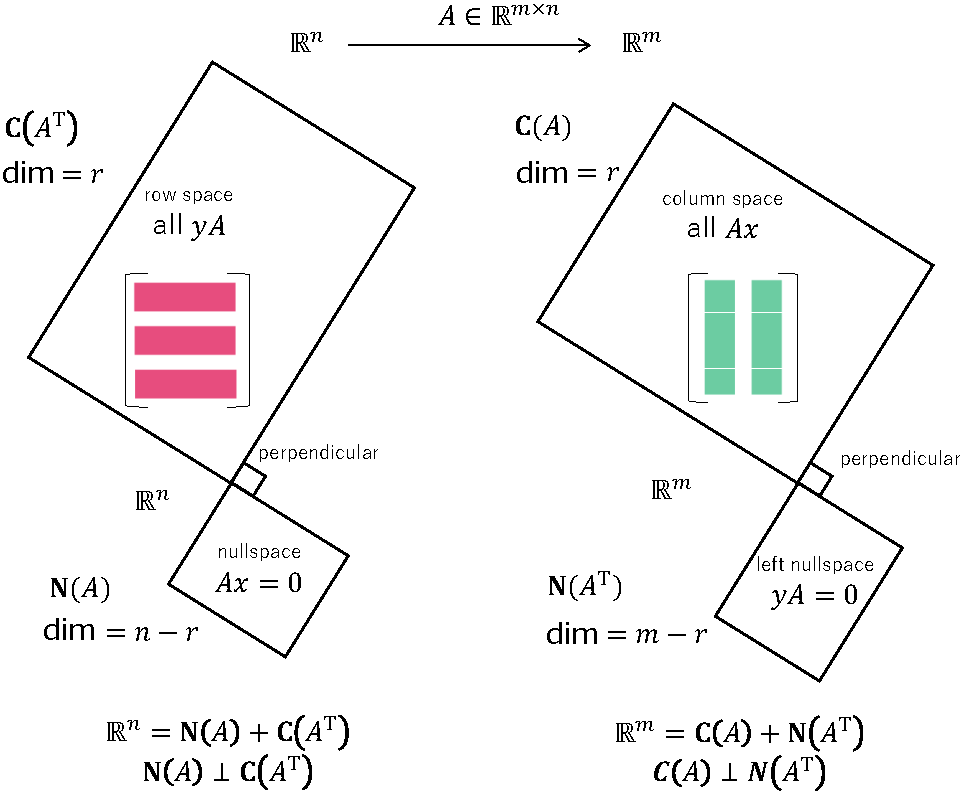
\includegraphics[width=13cm,height=10cm]{"figure/Question/四个子空间.pdf"}
	\caption{四个子空间}
\end{figure} 
\begin{solution}

	(1). 我们可以知道矩阵$A$的零空间为$N(A)=R^{n}$,我们可以得到$A$的行空间$R(A)=0$,$A=0$
	
	(2). 当$A$为反对称矩阵时,我们可以得到$\xi^{T}A\xi=0$
	
	(3). 我们不妨取$B=E$,可以得到$A=0$,矩阵$A$只能为零矩阵,在$A=0$时,任意的$n$阶矩阵$B$满足$AB=0$
	
	(4). 同$(3)$,取$B=E$,可以得到$A=0$,矩阵$A$只能为零矩阵,在$A=0$时,任意的$n$阶矩阵$B$满足$B^{T}AB=0$
\end{solution}
\myspace{1}

2. 设函数$f(x)$在$(\dfrac{1}{2},+\infty)$上可导,且$\lim\limits_{h\to 0}\dfrac{f[(x+h)^2]-f(x^2+h)}{h}=1$,$f(1)=1$,求$f(x)$
\myspace{1}
\begin{solution}

	原极限等价于:  
	\begin{eqnarray*}
		I&=&\lim\limits_{h\to 0}\dfrac{f[(x+h)^2]-f(x^2+h)}{h}\\
		&=&\lim\limits_{h\to 0}\dfrac{f[(x+h)^2]-f(x^2)+f(x^2)-f(x^2+h)}{h}\\
		&=&\lim\limits_{h\to 0}\dfrac{f[(x+h)^2]-f(x^2)}{h}+\lim\limits_{h\to 0}\dfrac{f(x^2)-f(x^2+h)}{h}\\
		&=&[f(x^2)]'-f'(x^2)\\
		&=&(2x-1)f'(x^2)\\
		&=&1
	\end{eqnarray*}

	我们得到:  
	$$f'(x^2)=\dfrac{1}{2x-1}\Rightarrow 2xf'(x^2)=\dfrac{2x}{2x-1}\Rightarrow f(x^2)=x+\dfrac{1}{2}\ln(2x-1)+C$$
	
	我们由$f(1)=1\Rightarrow C=0\Rightarrow f(x^2)=x+\dfrac{1}{2}\ln(2x-1)$
	
	我们得到$f(x)=\sqrt{x}+\dfrac{1}{2}\ln(2\sqrt{x}-1)$
\end{solution}
\myspace{1}

\textcolor{blue}{August 9}

1. $f(x)$在$[0,1]$上导函数连续,$f(0)=f(1)=0$,证明:  $\int_{0}^{1}f^{2}(x)dx\leq \dfrac{1}{8}\int_{0}^{1}[f'(x)]^2dx$
\myspace{1}
\begin{theorem}[积分形式柯西不等式]
	$$\left[ \int_{a}^{b}f(x)g(x)dx\right] ^2\leq \int_{a}^{b}f^2(x)dx\int_{a}^{b}g^{2}(x)dx$$
	
	我们知道$\forall t\in\mathbb{R}$,我们有:  
	$$\left[ tf(x)-g(x)\right]^2\geq 0\Rightarrow t^2f^{2}(x)-2tf(x)g(x)+g^{2}(x)\geq 0$$
	
	我们对上式子两边在区间$[a,b]$上积分,可以得到:  
	$$t^2\int_{a}^{b}f^{2}(x)dx-2t\int_{a}^{b}f(x)g(x)dx+\int_{a}^{b}g^{2}(x)dx\geq 0$$
	
	我们可以得到一个关于$t$的一元二次方程方程:  
	$$At^2+Bt+C\geq 0,\text{其中}\left\lbrace
	\begin{array}{l}
		A=\int_{a}^{b}f^{2}(x)dx\\
		B=-2\int_{a}^{b}f(x)g(x)dx\\
		C=\int_{a}^{b}g^{2}(x)dx
	\end{array}
	\right. \Rightarrow B^2-4AC\leq 0$$
	
	我们得到:  $$4\left[ \int_{a}^{b}f(x)g(x)dx\right]^2-4\int_{a}^{b}f^{2}(x)dx\int_{a}^{b}g^{2}(x)dx\leq 0 
	$$
	$$\left[ \int_{a}^{b}f(x)g(x)dx\right] ^2\leq \int_{a}^{b}f^2(x)dx\int_{a}^{b}g^{2}(x)dx$$
\end{theorem}
\begin{solution}

	我们知道:  $\left\lbrace
	\begin{array}{l}
		f(x)=\int_{0}^{x}f'(t)dt\\
		f(x)=\int_{1}^{x}f'(t)dt
	\end{array}
	\right. $
	我们有:  $$\int_{0}^{1}f^{2}(x)dx=\left\lbrace
	\begin{array}{l}
		\int_{0}^{1}\left[\int_{0}^{x}f'(t)dt \right]^2dx\leq \int_{0}^{1}[\int_{0}^{x}1^2dt\int_{0}^{x}|f'(t)|^2dt]dx\\
		\int_{0}^{1}\left[\int_{1}^{x}f'(t)dt \right]^2dx\leq \int_{0}^{1}[\int_{1}^{x}1^2dt\int_{0}^{x}|f'(t)|^2dt]dx
	\end{array}
	\right.$$
	
	我们可以得到:  
	\begin{eqnarray*}
		\int_{0}^{1}f^{2}(x)dx&=&\int_{0}^{\frac{1}{2}}f^{2}(x)dx+\int_{\frac{1}{2}}^{1}f^{2}(x)dx\\
		&=&\int_{0}^{\frac{1}{2}}\left[\int_{0}^{x}f'(t)dt \right]^2dx+\int_{\frac{1}{2}}^{1}\left[\int_{x}^{1}f'(t)dt \right]^2dx\\
		&\leq&\int_{0}^{\frac{1}{2}}[\int_{0}^{x}1^2dt\int_{0}^{x}|f'(t)|^2dt]dx+\int_{\frac{1}{2}}^{1}[\int_{x}^{1}1^2dt\int_{x}^{1}|f'(t)|^2dt]dx\\
		&\leq&\int_{0}^{\frac{1}{2}}[x\int_{0}^{x}|f'(t)|^2dt]dx+\int_{\frac{1}{2}}^{1}[(1-x)\int_{x}^{1}|f'(t)|^2dt]dx\\
		&=&\int_{0}^{\frac{1}{2}}|f'(t)|^2dt\int_{t}^{\frac{1}{2}}xdx+\int_{\frac{1}{2}}^{1}|f'(t)|^2dt\int_{\frac{1}{2}}^{t}(1-x)dx\\
		&=&(\dfrac{1}{8}-\dfrac{t^2}{2})\int_{0}^{\frac{1}{2}}|f'(t)|^2dt+(t-\dfrac{t^2}{2}-\dfrac{3}{8})\int_{\frac{1}{2}}^{1}|f'(t)|^2dt\\
		&=&\dfrac{1}{8}\int_{0}^{\frac{1}{2}}|f'(t)|^2dt+\dfrac{1}{8}\int_{\frac{1}{2}}^{1}|f'(t)|^2dt\\
		&=&\dfrac{1}{8}\int_{0}^{1}[f'(x)]^2dx
	\end{eqnarray*}
\end{solution}
\myspace{1}

2. 求$\lim\limits_{n\to+\infty}\left[\sqrt{n}(\sqrt{n+1}-\sqrt{n})+\dfrac{1}{2} \right]^{\dfrac{\sqrt{n+1}+\sqrt{n}}{\sqrt{n+1}-\sqrt{n}}} $
\myspace{1}
\begin{solution}

	原极限等价于:  
	\begin{eqnarray*}
		I&=&e^{\lim\limits_{n\to+\infty}\dfrac{\ln\left( 1+\dfrac{\sqrt{n}-\sqrt{n+1}}{2(\sqrt{n+1}+\sqrt{n})}\right)}{(\sqrt{n+1}-\sqrt{n})^2}}\\
		&=&e^{\lim\limits_{n\to+\infty}\dfrac{\dfrac{\sqrt{n}-\sqrt{n+1}}{2(\sqrt{n+1}+\sqrt{n})}}{(\sqrt{n+1}-\sqrt{n})^2}}\\
		&=&e^{\lim\limits_{n\to+\infty}-\dfrac{1}{2}}\\
		&=&e^{-\frac{1}{2}}
	\end{eqnarray*}
\end{solution}
\myspace{1}

\textcolor{blue}{August 10}

1. 设可导函数$y=y(x)$由方程$\sin x-\int_{x}^{y}\varphi(u)du=0$所确定,其中可导函数$\varphi(u)>0$,且$\varphi(0)=\varphi'(0)=1$,求$y''(0)$
\myspace{1}
\begin{solution}

	我们可以得到:  当$x=0$时,$\int_{0}^{y}\varphi(u)du=0$,且$\varphi(u)>0$,我们得到$y=0$.
	
	我们对方程$\sin x-\int_{x}^{y}\varphi(u)du=0$两边对$x$求导得到:  
	$$\left\lbrace
	\begin{array}{l}
		\cos x-[\varphi(y)y'-\varphi(x)]=0\\
		-\sin x-[\varphi'(y)y'^2+\varphi(y)y''-\varphi'(x)]=0
	\end{array}
	\right. \Rightarrow \left\lbrace
	\begin{array}{l}
		1-y'(0)\varphi(0)+\varphi(x)=0\\
		-\varphi'(0)y'(0)^2-y''(0)\varphi(0)+\varphi'(0)=0
	\end{array}
	\right. \Rightarrow \left\lbrace
	\begin{array}{l}
		y'(0)=2\\
		y''(0)=-3
	\end{array}
	\right. $$
\end{solution}
\myspace{1}

2. 设$a_{n}=\int_{0}^{1}\dfrac{x^n}{1+x}dx$

(1).证明:  $\dfrac{1}{2(n+1)}\leq a_{n}\leq \dfrac{1}{2n},\ n=1,2,\cdots$

(2). 证明:  级数$\sum\limits_{n=1}^{+\infty}(-1)^{n-1}(\dfrac{1}{2n}-\int_{0}^{1}\dfrac{x^n}{1+x}dx)$绝对收敛.
\myspace{1}
\begin{solution}

	(1). 我们有:  $$\left\lbrace
	\begin{array}{l}
		\dfrac{x^n}{1+x}\geq \dfrac{x^n}{2},\ x\in(0,1)\\
		\dfrac{x^n}{1+x}=\dfrac{x}{1+x}x^{n-1}\leq\dfrac{x^{n-1}}{2},\ x\in(0,1)
	\end{array}
	\right. \Rightarrow \int_{0}^{1}\dfrac{x^n}{2}dx\leq \int_{0}^{1}\dfrac{x^n}{1+x}dx\leq \int_{0}^{1}\dfrac{x^{n-1}}{2}dx$$
	
	我们有:  $$\left\lbrace
	\begin{array}{l}
		\int_{0}^{1}\dfrac{x^n}{2}dx=\dfrac{x^{n+1}}{2(n+1)}|_{0}^{1}=\dfrac{1}{2(n+1)}\\
		\int_{0}^{1}\dfrac{x^{n-1}}{2}dx=\dfrac{x^{n}}{2n}|_{0}^{1}=\dfrac{1}{2n}
	\end{array}
	\right. $$
	
	我们证明了:  $\dfrac{1}{2(n+1)}\leq a_{n}\leq \dfrac{1}{2n},\ n=1,2,\cdots$
	
	(2). 我们不妨设$b_{n}=\dfrac{1}{2n}-a_{n}=\dfrac{1}{2n}-\int_{0}^{1}\dfrac{x^n}{1+x}dx$.
	
	我们由$(1)$可得:  $|b_{n}|\leq \dfrac{1}{2n}-\dfrac{1}{2(n+2)}=\dfrac{1}{2n^2+4n}<\dfrac{1}{2n^2}$
	
	我们知道级数$\sum\limits_{n=1}^{+\infty}\dfrac{1}{2n^2}$收敛,由比较判别法我们可知级数$\sum\limits_{n=1}^{+\infty}b_{n}$收敛,原级数绝对收敛.
\end{solution}
\myspace{1}

\textcolor{blue}{August 11}

1. 设$x=x(y)$是函数$y=\ln x+e^x$的反函数,求$\dfrac{d^2x}{dy^2}$.
\myspace{1}
\begin{solution}

	我们有:  $\left\lbrace
	\begin{array}{l}
		y=f(x)\\
		x=g(y)
	\end{array}
	\right. \Rightarrow \left\lbrace
	\begin{array}{l}
		y'(x)=f'(x)\\
		1=f'(x)g'(y)
	\end{array}
	\right. \Rightarrow g'(y)=\dfrac{1}{f(x)}$
	
	我们有:  $f(x)=\ln x+e^x\Rightarrow f'(x)=e^x+\dfrac{1}{x}$
	
	我们得到:  $g'(y)=\dfrac{dx}{dy}=\dfrac{1}{f(x)}=\dfrac{x}{1+xe^x}$
	
	我们有:  
	$$\dfrac{d^2x}{dy^2}=\dfrac{\dfrac{dx}{dy}}{dx}\dfrac{dx}{dy}=\dfrac{x-x^3e^x}{(1+xe^x)^3}$$
\end{solution}
\myspace{1}

2. 设$a_{0}=1,a_{1}=0$,$a_{n+1}=\dfrac{1}{n+1}(na_{n}+a_{n-1})\ (n=1,2,3\cdots)$,$S(x)$为幂级数$\sum\limits_{n=0}^{+\infty}a_{n}x^{n}$的和函数.

(1).证明:  幂级数$\sum\limits_{n=0}^{+\infty}a_{n}x^n$的收敛半径不小于$1$.

(2).证明:  $(1-x)S'(x)-xS(x)=0,\ x\in(-1,1)$,并求出$S(x)$的表达式.
\myspace{1}
\begin{solution}

	(1). 我们由$a_{n+1}=\dfrac{1}{n+1}(na_{n}+a_{n-1})$得到:  
	$$a_{n+1}-a_{n}=-\dfrac{1}{n+1}(a_{n}-a_{n-1})$$
	
	我们不妨设$b_{n}=a_{n}-a_{n-1}\Rightarrow b_{n+1}=-\dfrac{1}{n+1}b_{n},\ b_{1}=a_{1}-a_{0}=-1$
	
	我们有:  $$\left\lbrace
	\begin{array}{l}
		b_{n}=-\dfrac{1}{n}b_{n-1}\\
		b_{n-1}=-\dfrac{1}{n-1}b_{n-2}\\
		\cdots\\
		b_{2}=-\dfrac{1}{2}b_{1}\\
		b_{1}=-1
	\end{array}
	\right. \Rightarrow b_{n}=\dfrac{(-1)^{n}}{n!}$$
	
	我们由累加法可以得到:  $a_{n}=\left\lbrace
	\begin{array}{l}
		a_{0}+\sum\limits_{k=1}^{n}b_{k}=\sum\limits_{k=0}^{n}\dfrac{(-1)^k}{k!},\ n\geq 1\\
		1,\ n=0
	\end{array}
	\right. \Rightarrow a_{n}=\sum\limits_{k=0}^{n}\dfrac{(-1)^k}{k!}$
	
	我们利用根值审敛法:  
	$$\rho=\lim\limits_{n\to+\infty}\sqrt[n]{a_{n}}=e^{\lim\limits_{n\to +\infty}\dfrac{\ln(\sum\limits_{k=0}^{n}\dfrac{(-1)^k}{k!})}{n}}=1$$
		
	我们得到级数的收敛半径:  $r=\dfrac{1}{\rho}=1$,幂级数$\sum\limits_{n=0}^{+\infty}a_{n}x^n$的收敛半径不小于$1$.

	(2). 我们有:  $S(x)=\sum\limits_{n=0}^{+\infty}a_{n}x^{n}$,我们得到:  
	$$\left\lbrace
	\begin{array}{l}
		S'(x)=\sum\limits_{n=1}^{+\infty}na_{n}x^{n-1}=\sum\limits_{n=0}^{+\infty}(n+1)a_{n+1}x^{n}\\
		S(x)=\sum\limits_{n=0}^{+\infty}a_{n}x^{n}
	\end{array}
	\right.$$
	
	$$a_{n+1}=\dfrac{1}{n+1}(na_{n}+a_{n-1})\Rightarrow (n+1)a_{n+1}=na_{n}+a_{n-1}\Rightarrow (n+2)a_{n+2}=(n+1)a_{n+1}=a_{n}$$
	
	我们得到:  
	\begin{eqnarray*}
		(1-x)S'(x)-xS(x)&=&(1-x)\sum\limits_{n=0}^{+\infty}(n+1)a_{n+1}x^{n}-x\sum\limits_{n=0}^{+\infty}a_{n}x^{n}\\
		&=&\sum\limits_{n=0}^{+\infty}(n+1)a_{n+1}x^{n}-\sum\limits_{n=0}^{+\infty}[(n+1)a_{n+1}+a_{n}]x^{n+1}\\
		&=&a_{1}+\sum\limits_{n=1}^{+\infty}(n+1)a_{n+1}x^{n}-\sum\limits_{n=0}^{+\infty}[(n+1)a_{n+1}+a_{n}]x^{n+1}\\
		&=&\sum\limits_{n=0}^{+\infty}(n+2)a_{n+2}x^{n+1}-\sum\limits_{n=0}^{+\infty}[(n+1)a_{n+1}+a_{n}]x^{n+1}\\
		&=&\sum\limits_{n=0}^{+\infty}[(n+2)a_{n+2}-(n+1)a_{n+1}-a_{n}]x^{n+1}\\
		&=&0
	\end{eqnarray*}
	
	我们得到:  
	$$(1-x)S'(x)-xS(x)=0\Rightarrow \dfrac{S'(x)}{S(x)}=\dfrac{x}{1-x}\Rightarrow S(x)=\dfrac{C_{1}}{e^x(1-x)}$$
	
	我们有$S(0)=1\Rightarrow C_{1}=1$,因此$S(x)=\dfrac{1}{e^x(1-x)},\ x\in(-1,1)$
	
\end{solution}
\myspace{1}

\textcolor{blue}{August 12}

1. 设$y=y(x)$由$e^y\sin t-y+1=0$和$x=\left\lbrace
\begin{array}{l}
	\dfrac{e^t-1}{t},\ t\neq 0\\
	1,\ t=0
\end{array}
\right. $所确定,求$\dfrac{d^2y}{dx^2}|_{t=0}$
\myspace{1}
\begin{solution}

	我们知道:  当$t=0$时,$\left\lbrace
	\begin{array}{l}
		x=1\\y=1
	\end{array}
	\right. $,我们由:  
	$$x(t)=\left\lbrace
	\begin{array}{l}
		\dfrac{e^t-1}{t},\ t\neq 0\\
		1,\ t=0
	\end{array}
	\right. \Rightarrow x(t)=1+\dfrac{t}{2}+\dfrac{t^2}{6}+\dfrac{t^3}{24}+\cdots\Rightarrow \left\lbrace
	\begin{array}{l}
		x'(0)=\dfrac{1}{2}\\
		x''(0)=\dfrac{1}{3}
	\end{array}
	\right. $$
	
	我们由:  $e^y\sin t-y+1=0\Rightarrow e^{y(t)}\sin t-y(t)+1=0$得到:  
	$$\left\lbrace
	\begin{array}{l}
		e^{y(t)}\cos t+y'(t)e^{y(t)}\sin t-y'(t)=0\\
		y'(t)e^{y(t)}\cos t-e^{y(t)}\sin t+\left\lbrace [y'(t)]^2e^{y(t)}+y''(t)e^{y(t)}\right\rbrace \sin x+\cos x\left[y'(t)e^{y(t)} \right]-y''(t)=0
	\end{array}
	\right.$$
	$$\left\lbrace
	\begin{array}{l}
		y'(0)=e\\
		y''(0)=2e^2
	\end{array}
	\right. $$
	
	我们由参数方程二阶导数公式:  
	$$\dfrac{d^2y}{dx^2}|_{t=0}=\dfrac{y''(t)x'(t)-x''(t)y'(t)}{[x'(t)]^3}|_{t=0}=8e^2-\dfrac{8e}{3}$$
	
\end{solution}
\myspace{1}

2. 下列命题正确的是:  
\begin{itemize}
	\item \hl{A}. 设$A$为$3$阶矩阵,若$A$的特征值$\lambda_{1}\lambda_{2}\neq 0,\lambda_{3}=0$,则$r(A)=2$
	\item \hl{B}. 设$A$为$3$阶非零矩阵,若$A^2=0$,则$r(A)=1$
	\item C. 设$A,B$为$3$阶矩阵,若$A$与$B$等价,则$|A|=|B|$
	\item D. 设$A,B$为$3$阶实对称矩阵,若$A$与$B$合同,则$|A|=|B|$
\end{itemize}
\myspace{1}
\begin{solution}

	(A). 我们可以得到矩阵$A\sim diag\{\lambda_{1},\lambda_{2},\lambda_{3}\}$,对角矩阵的秩和矩阵$A$的秩相同,$r(A)=2$
	
	(B). $A^2=0\Rightarrow 2r(A)\leq 3\Rightarrow r(A)=1$
	
	(C). $A$与$B$等价$\Rightarrow r(A)=r(B)$
	
	(D). $A$与$B$合同$\Rightarrow A=P^{T}BP$
\end{solution}
\myspace{1}

\textcolor{blue}{August 13}

1. 已知$f(x)=\left\lbrace
\begin{array}{l}
	\lim\limits_{n\to +\infty}\left( 1+\dfrac{2nx+x^2}{2n^2}\right)^{-n},\ x\neq 0\\
	\lim\limits_{n\to +\infty}2\left[ \dfrac{n}{(n+1)^2}+\dfrac{n}{(n+2)^2}+\cdots+\dfrac{n}{(n+n)^2}\right],\ x=0  
\end{array}
\right. $,求$\int f(x)dx$
\myspace{1}
\begin{solution}

	当$x\neq 0$时:  
	\begin{eqnarray*}
		f(x)&=&\lim\limits_{n\to +\infty}\left( 1+\dfrac{2nx+x^2}{2n^2}\right)^{-n}\\
		&=&e^{\lim\limits_{n\to +\infty}(-n)\dfrac{2nx+x^2}{2n^2}}\\
		&=&e^{-x}
	\end{eqnarray*}

	当$x=0$时:  
	\begin{eqnarray*}
		f(x)&=&\lim\limits_{n\to +\infty}2\left[ \dfrac{n}{(n+1)^2}+\dfrac{n}{(n+2)^2}+\cdots+\dfrac{n}{(n+n)^2}\right]\\
		&=&2\lim\limits_{n\to +\infty}\dfrac{1}{n}\left[ \dfrac{1}{(1+\dfrac{1}{n})^2}+\dfrac{1}{(1+\dfrac{2}{n})^2}+\cdots+\dfrac{1}{(1+\dfrac{n}{n})^2}\right]\\
		&=&2\int_{0}^{1}\dfrac{1}{(1+x)^2}dx\\
		&=&2(1-\dfrac{1}{2})\\
		&=&1
	\end{eqnarray*}

	我们得到:  $f(x)=e^{-x}\Rightarrow \int f(x)dx=-e^{-x}+C$
\end{solution}
\myspace{1}

2. 已知函数$f(x)=x^2\ln(1-x)$,当$n\geq 3$时,求$f^{(n)}(0)$
\myspace{1}
\begin{solution}

	我们利用$\ln(1-x)$的泰勒展开式:  
	$$\ln(1-x)=-x-\dfrac{x^2}{2}-\dfrac{x^3}{3}-\cdots-\dfrac{x^n}{n}-\cdots$$
	
	我们可以得到:  
	$$f(x)=-x^3-\dfrac{x^4}{2}-\dfrac{x^5}{3}-\cdots-\dfrac{x^n+2}{n}-\cdots$$
	
	我们有:  
	$$\left\lbrace
	\begin{array}{l}
		f'(0)=0\\
		f''(0)=0\\
		f^{(3)}(0)=-6\\
		f^{(4)}(0)=-\dfrac{4!}{2}\\
		\cdots\cdots
	\end{array}
	\right. \Rightarrow f^{(n)}(0)=-\dfrac{n!}{n-2},\ n\geq 3$$
\end{solution}
\myspace{1}

\textcolor{blue}{August 14}

1. 设$f(x)$在$[0,1]$上可导,$f(0)=f(1)=-2$,证明:  $\exists \xi\in(0,1),\ s.t. f'(\xi)-f(\xi)=\xi$
\myspace{1}
\begin{solution}

	我们构造辅助函数:  $F(x)=e^{-x}\left[ f(x)+x+1\right]$,我们有:  
	$$F(0)=-1,\ F(1)=0,\ F'(x)=e^{-x}\left[ f'(x)-f(x)-x\right]$$
	
	我们由积分中值定理可以得到:  
	$$\exists \eta\in(0,1),\ s.t. \int_{0}^{1}f(x)dx=f(\eta)\Rightarrow \exists \eta\in(0,1),\ s.t. f(\eta)=0$$
	
	我们有:  
	$$F(\eta)=e^{-\eta}\left[ f(\eta)+\eta+1\right]=e^{-\eta}(\eta+1)>0$$
	
	我们根据零点定理,可知:  $\exists \delta\in(0,\eta),\ s.t. F(\delta)=0$.
	
	我们对$F(x)$在区间$[\delta,1]$上使用罗尔定理可以得到:  
	$$\exists\xi\in(\delta,1),\ s.t. F'(\xi)=e^{-\xi}\left[ f'(\xi)-f(\xi)-\xi\right]=0\Rightarrow f'(\xi)-f(\xi)=\xi$$
	
	综上所述,我们得到:  $\exists \xi\in(0,1),\ s.t. f'(\xi)-f(\xi)=\xi$
\end{solution}
\myspace{1}

2. 设数列$\{u_{n}\}$满足$u_{1}=1,\ u_{n+1}=\dfrac{u_{n}+3}{u_{n}+1},\ (n=1,2,\cdots)$,试证明数列$\{u_{n}\}$收敛,并求其极限.
\myspace{1}
\begin{solution}

	我们有:
	$$u_{1}=1,\ u_{2}=2,\ u_{3}=\dfrac{5}{3},\ u_{4}=\dfrac{7}{4},\cdots\ (u_{n}>0)$$
	
	我们发现数列$\{u_{n}\}$不是单调数列,我们从奇数项和偶数项入手:
	$$\left\lbrace
	\begin{array}{l}
		u_{2k+2}=\dfrac{u_{2k+1}+3}{u_{2k+1}+1}=\dfrac{\frac{u_{2k}+3}{u_{2k}+1}+3}{\frac{u_{2k}+3}{u_{2k}+1}+1}=2-\dfrac{1}{u_{2k}+2}\\
		u_{2k+1}=\dfrac{u_{2k}+3}{u_{2k}+1}=\dfrac{\frac{u_{2k-1}+3}{u_{2k-1}+1}+3}{\frac{u_{2k-1}+3}{u_{2k-1}+1}+1}=2-\dfrac{1}{u_{2k-1}+2}
	\end{array}
	\right. \Rightarrow f(x)=2-\dfrac{1}{x+2}\text{单调递增}$$
	
	我们首先证明数列$\{u_{2k-1}\}$极限存在:  
	
	(1). 当$n=1$时,$u_{1}<u_{3}$.
	
	(2). 当$n=k$时,假设$u_{2k-1}<u_{2k+1}$
	
	(3). 当$n=k+1$时,$u_{2k-1}<u_{2k+1}\Rightarrow f(u_{2k-1})<f(u_{2k+1})\Rightarrow u_{2k+1}<u_{2k+3}$
	
	数列$\{u_{2k-1}\},(k=1,2,\cdots)$单调递增,且$u_{2k-1}<2$
	
	我们继续证明数列$\{u_{2k}\}$极限存在:  
	
	(1). 当$n=1$时,$u_{2}>u_{4}$.
	
	(2). 当$n=k$时,假设$u_{2k}>u_{2k+2}$
	
	(3). 当$n=k+1$时,$u_{2k}>u_{2k+2}\Rightarrow f(u_{2k})>f(u_{2k+2})\Rightarrow u_{2k+2}<u_{2k+4}$
	
	数列$\{u_{2k}\},(k=1,2,\cdots)$单调递减少,且$u_{2k}>\dfrac{3}{2}$
	
	我们不妨假设:  $$\left\lbrace
	\begin{array}{l}
		\lim\limits_{k\to +\infty}u_{2k-1}=A\\
		\lim\limits_{k\to +\infty}u_{2k}=B\\
	\end{array}
	\right. \Rightarrow \left\lbrace
	\begin{array}{l}
		A=\dfrac{B+3}{B+1}\\
		B=\dfrac{A+3}{A+1}
	\end{array}
	\right. \Rightarrow A=B=\sqrt{3}$$
	
	我们可以得到:  
	
	(1). $\forall \varepsilon>0$,$\exists N_{1}>0$,当$n=2k-1>N_{1}$时,我们有:$|u_{2k-1}-\sqrt{3}|<\varepsilon$.
	
	(2). $\forall \varepsilon>0$,$\exists N_{2}>0$,当$n=2k>N_{2}$时,我们有:$|u_{2k}-\sqrt{3}|<\varepsilon$.
	
	(3). 取$N=\text{max}\{N_{1},N_{2}\}$,$\forall \varepsilon>0$,$\exists N>0$,当$n>N$时,我们有:$|u_{n}-\sqrt{3}|<\varepsilon$.
	
	综上所述,我们证明数列$\{u_{n}\}$收敛,极限为$\sqrt{3}$.
\end{solution}
\myspace{1}

\section{Week \Rmnum{3}}
\textcolor{cyan}{August 15}

1. $f(x)=\int_{1}^{x}\dfrac{\arctan t}{(1+t^2)^{\frac{3}{2}}\ln(1+t^2)}dt$,求$\int_{0}^{1}\dfrac{x}{1+x^2}f(x)dx$
\myspace{1}
\begin{solution}

	原定积分等价于:  
	\begin{eqnarray*}
		I&=&\int_{0}^{1}\dfrac{f(x)}{2}d(\ln(1+x^2))\\
		&=&\dfrac{f(x)\ln(1+x^2)}{2}|_{x=0}^{x=1}-\int_{0}^{1}\dfrac{\ln(1+x^2)}{2}d(f(x))\\
		&=&-\int_{0}^{1}\dfrac{\arctan x}{2(1+x^2)^{\frac{3}{2}}}dx\\
		&=&-\dfrac{1}{2}\int_{0}^{\frac{\pi}{4}}\theta\cos\theta d\theta\\
		&=&-\dfrac{1}{2}\theta\sin\theta|_{\theta=0}^{\theta=\frac{\pi}{4}}-\dfrac{1}{2}\int_{0}^{\frac{\pi}{4}}\sin \theta d\theta\\
		&=&-\dfrac{\sqrt{2}\pi}{16}+\dfrac{2-\sqrt{2}}{4}
	\end{eqnarray*}
\end{solution}
\myspace{1}

2. 设$f(x)=\dfrac{1}{1+2x+4x^2}$,求$f^{(100)}(0)$
\myspace{1}
\begin{solution}

	$$f(x)=\dfrac{1-2x}{(1-2x)(4x^2+2x+1)}=\dfrac{1-2x}{1-(2x)^3}$$
	$$\dfrac{1}{1-(2x)^3}=1+(2x)^3+(2x)^6+(2x)^9+\cdots+(2x)^{3n}$$
	
	我们得到:$$f(x)=(1-2x)\sum\limits_{n=0}^{+\infty}(2x)^{3n}=\sum\limits_{n=0}^{+\infty}(2x)^{3n}-\sum\limits_{n=0}^{+\infty}(2x)^{3n+1}$$
	$$f(x)=f(0)+f'(0)x+\cdots+\dfrac{f^{(n)}(0)}{n!}x^n$$
	
	$\dfrac{f^{(100)}(0)}{100!}$是$f(x)$中$x^{100}$前面的系数,我们可以得到:  
	$$f^{(100)}(0)=-2^{100}\times100!$$
\end{solution}
\myspace{1}

\textcolor{cyan}{August 16}

1. 证明:  在区间$(0,2)$内存在三个不同的点$x_{1},x_{2},x_{3}$,使得$\dfrac{1-\ln(1+x_{1})}{(1+x_{1})^2}x_{3}=\dfrac{1-\ln(1+x_{2})}{(1+x_{2})^2}(2-x_{3})$
\myspace{1}
\begin{solution}

	我们构造辅助函数:  $f(x)=\dfrac{\ln(1+x)}{1+x}$,我们有:  
	$$\left\lbrace 
	\begin{array}{l}
		f'(x)=\dfrac{1-\ln(1+x)}{(1+x)^2}\\
		f(0)=0\\
		f(2)=\dfrac{\ln 3}{3}
	\end{array}
	\right. $$
	
	我们不妨假设$\exists x_{3}\in(0,2), f(x_{3})=A$,我们分别在区间$(0,x_{3})$和区间$(x_{3},2)$上使用拉格朗日中值定理可以得到:  
	$$\left\lbrace 
	\begin{array}{l}
		\exists x_{1}\in(0,x_{3}),\ s.t. \dfrac{f(x_{3})-f(0)}{x_{3}}=f'(x_{1})=\dfrac{1-\ln(1+x_{1})}{(1+x_{1})^2}\\
		\exists x_{2}\in(x_{3},2),\ s.t. \dfrac{f(2)-f(x_{3})}{2-x_{3}}=f'(x_{2})=\dfrac{1-\ln(1+x_{2})}{(1+x_{2})^2}
	\end{array}
	\right. $$
	
	我们令$f(x_{3})-f(0)=f(2)-f(x_{3})\Rightarrow A=f(2)-A\Rightarrow f(x_{3})=A=\dfrac{f(2)}{2}=\dfrac{\ln 3}{6}$时,我们可以得到:  $$\dfrac{1-\ln(1+x_{1})}{(1+x_{1})^2}x_{3}=\dfrac{1-\ln(1+x_{2})}{(1+x_{2})^2}(2-x_{3})$$
	
	综上所述,我们可以得到:  在区间$(0,2)$内存在三个不同的点$x_{1},x_{2},x_{3}$,使得$\dfrac{1-\ln(1+x_{1})}{(1+x_{1})^2}x_{3}=\dfrac{1-\ln(1+x_{2})}{(1+x_{2})^2}(2-x_{3})$
\end{solution}
\myspace{1}

2. 设$y=\dfrac{\arcsin x}{\sqrt{1-x^2}}$

(1). 证明:  $(1-x^2)y^{(n+1)}-(2n+1)xy^{(n)}-n^2y^{(n-1)}=0(n\geq 1)$;

(2). 求$y^{(n)}(0)$
\myspace{1}
\begin{solution}

	(1). 我们对$f(x)$求导可以得到:  
	$$f'(x)=\dfrac{1+\dfrac{x\arcsin x}{\sqrt{1-x^2}}}{1-x^2}\Rightarrow f'(x)=\dfrac{1+xf(x)}{1-x^2}\Rightarrow (1-x^2)f'(x)-xf(x)-1=0$$
	
	我们令$g(x)=(1-x^2)f'(x)-xf(x)-1$,我们利用莱布尼兹公式可以得到:  
	$$g^{(n)}(x)=\sum\limits_{k=0}^{n}C_{n}^{k}(1-x^2)^{(k)}f^{(n-k+1)}(x)-\sum\limits_{k=0}^{n}C_{n}^{k}(x)^{(k)}f^{(n-k)}=0$$
	
	当$k\geq 3$时,$(1-x^2)^{(k)}=0$;当$k\geq 2$时,$x^{(k)}=0$,我们有:  
	$$g^{(n)}(x)=(1-x^2)f^{(n+1)}(x)-2nxf^{(n)}(x)-n(n-1)f^{(n-1)}(x)-xf^{(n)}(x)-nf^{(n-1)}(x)=0$$
	
	我们得到:  
	$$(1-x^2)f^{(n+1)}(x)-(2n+1)xf^{(n)}(x)-n^2f^{(n-1)}(x)=0$$
	
	综上所述,我们得到:  $(1-x^2)y^{(n+1)}-(2n+1)xy^{(n)}-n^2y^{(n-1)}=0(n\geq 1)$
	
	(2). 我们将$x=0$代入上面式子可以得到:  
	$$\left\lbrace 
	\begin{array}{l}
		y^{(n)}=(n-1)^2y^{(n-2)}\\
		y(0)=0\\
		y^{(1)}(0)=1
	\end{array}
	\right. \Rightarrow y^{(n)}(0)=\left\lbrace 
	\begin{array}{l}
		0,\ n\text{为偶数},n=2k(k=0,1,\cdots)\\
		(2k!!)^2,\ n\text{为奇数},n=2k+1(k=0,1,\cdots)
	\end{array}
	\right. $$
\end{solution}
\myspace{1}

\textcolor{cyan}{August 17}

1. 已知极限$\lim\limits_{t\to x}\left(\dfrac{\sin t}{\sin x} \right)^{\dfrac{x}{\sin t-\sin x}}$,记此极限为$f(x)$,求函数$f(x)$的间断点,并指出其类型.
\myspace{1}
\begin{solution}

	$$f(x)=e^{\lim\limits_{t\to x}\frac{x}{\sin t-\sin x}\ln(1+\frac{\sin t-\sin x}{\sin x})}=e^{\frac{x}{\sin x}}$$
	
	我们发现$f(x)$的间断点为$x=k\pi,\ k\in\mathbb{Z}$.
	
	(1). 当$k=0$时,我们有:
	$$\left\lbrace 
	\begin{array}{l}
		\lim\limits_{x\to 0^{+}}f(x)=e\\
		\lim\limits_{x\to 0^{-}}f(x)=e
	\end{array}
	\right. \Rightarrow x=0\text{是}f(x)\text{可去间断点}$$
	
	(2). 当$k\neq 0$时,我们有:
	$$\left\lbrace 
	\begin{array}{l}
		\lim\limits_{x\to k\pi^{+}}f(x)=+\infty\text{或者}0\\
		\lim\limits_{x\to 0^{-}}f(x)=0\text{或者}+\infty
	\end{array}
	\right. \Rightarrow x=k\pi\text{是}f(x)\text{无穷间断点}$$
\end{solution}
\myspace{1}

2. 证明:  $\int_{0}^{\pi}xa^{\sin x}dx\int_{0}^{\frac{\pi}{2}}a^{-\cos x}dx\geq \dfrac{\pi^3}{4}$
\myspace{1}
\begin{solution}

	我们由区间再现公式可以得到:
	$$\left\lbrace 
	\begin{array}{l}
		I_{1}=\int_{0}^{\pi}(\pi-t)a^{\sin t}dt\\
		2I_{1}=\pi\int_{0}^{\pi}a^{\sin t}dt\\
		I_{1}=\pi\int_{0}^{\frac{\pi}{2}}a^{\cos t}dt
	\end{array}
	\right. $$
	
	我们可以得到原定积分等价于:(柯西不等式)
	\begin{eqnarray*}
		\text{左边}&=&\pi\int_{0}^{\frac{\pi}{2}}a^{\cos x}dx\int_{0}^{\frac{\pi}{2}}a^{-\cos x}dx\\
		&=&\pi\int_{0}^{\frac{\pi}{2}}f^{2}(x)dx\int_{0}^{\frac{\pi}{2}}g^{2}(x)dx\\
		&\geq &\pi \left[ \int_{0}^{\frac{\pi}{2}}f(x)g(x)dx\right]^2\\
		&=&\dfrac{\pi^3}{4} 
	\end{eqnarray*}
\end{solution}
\myspace{1}

\textcolor{cyan}{August 18}

1. 设函数$f(x)=\left\lbrace
\begin{array}{l}
	x|x|,\ x\leq 0,\\
	x\ln x,\ x>0,
\end{array}
\right. $,\ $x=0$处$f(x)$的可导性判断、$x=0$是否为$f(x)$的极值点
\myspace{1}
\begin{solution}

	当$x=0$时,我们有$f(0)=0$,且我们有:  
	$$\left\lbrace
	\begin{array}{l}
		\lim\limits_{x\to 0^{+}}f(x)=\lim\limits_{x\to 0^{+}}x\ln x=0\\
		\lim\limits_{x\to 0^{-}}f(x)=\lim\limits_{x\to 0^{-}}(-x^2)=0
	\end{array}
	\right. \Rightarrow \lim\limits_{x\to 0}f(x)=f(0)\Rightarrow f(x)\text{在}x=0\text{处连续}$$
	
	我们有:  
	$$\left\lbrace
	\begin{array}{l}
		\lim\limits_{x\to 0^{+}}\dfrac{f(x)-f(0)}{x}=\ln x=-\infty\\
		\lim\limits_{x\to 0^{-}}\dfrac{f(x)-f(0)}{x}=-x=0
	\end{array}
	\right. \Rightarrow f(x)\text{在}x=0\text{处不可导}$$
	
	取$\varepsilon\in(0,1)$,当$x\in(-\varepsilon,0)$时,$f(x)=-x^2<f(0)=0$;当$x\in(0,\varepsilon)$时,$f(x)=x\ln x<f(0)=0$,$x=0$是$f(x)$的极大值点.
\end{solution}
\myspace{1}

2. 已知$f(x)=\prod\limits_{n=1}^{100}\left(\tan\dfrac{\pi x^n}{4}-n\right)$,求$f'(1)$
\myspace{1}
我们令$g(x)=\prod\limits_{n=2}^{100}\left(\tan\dfrac{\pi x^n}{4}-n\right)$,我们得到:$$f(x)=(\tan\dfrac{\pi x}{4}-1)g(x)$$
$$f'(x)=\dfrac{\pi}{4\cos^2\frac{\pi x}{4}}g(x)+g'(x)(\tan\dfrac{\pi x}{4}-1)$$
$$f'(1)=\dfrac{\pi}{2}g(1)=\dfrac{\pi}{2}\times(1-2)\times(1-3)\cdots\times(1-100)=-\dfrac{\pi}{2}99!$$
\myspace{1}

\textcolor{cyan}{August 19}

1. 已知函数$f(x)=\left\lbrace
\begin{array}{l}
	\int_{0}^{x}\cos\dfrac{1}{t}dt,\ x\neq 0\\
	0,\ x=0
\end{array}
\right. $,求$f'(0)$
\myspace{1}
\begin{solution}

	我们有:$\lim\limits_{x\to 0}f(x)=f(0)=0$,我们根据导数的定义可以得到:  
	\begin{eqnarray*}
		f'(0)&=&\lim\limits_{x\to 0}\dfrac{\int_{0}^{x}\cos\dfrac{1}{t}dt}{x}\\
		&=&\lim\limits_{x\to 0}-\dfrac{\int_{0}^{x}t^2d\sin\dfrac{1}{t}}{x}\\
		&=&\lim\limits_{x\to 0}\left[ -t\sin\dfrac{1}{t}|_{t=0}^{t=x}\right]+\lim\limits_{x\to 0}\dfrac{\int_{0}^{x}2t\sin\dfrac{1}{t}dt}{x}\\
		&=&0+2\lim\limits_{x\to 0}x\sin\dfrac{1}{x}\\
		&=&0
	\end{eqnarray*}

	综上所述,我们得到:$f'(0)=0$
\end{solution}
\myspace{1}

2. $f(x)$可导,且满足$x=\int_{0}^{x}f(t)dt+\int_{0}^{x}tf(t-x)dt$,求$f(x)$以及$\int_{-\frac{\pi}{4}}^{\frac{3\pi}{4}}|f(x)|^6dx$
\myspace{1}
\begin{solution}

	我们令$u=t-x,t=u+x$,我们得到:
	$$x=\int_{0}^{x}f(t)dt+\int_{-x}^{0}(u+x)f(u)du\Rightarrow x=\int_{0}^{x}f(t)dt+\int_{-x}^{0}uf(u)du+x\int_{-x}^{0}f(u)du$$
	
	我们对方程左右两边对$x$求导,得到:
	$$1=f(x)-xf(-x)+\int_{-x}^{0}f(u)du+xf(-x)\Rightarrow f(x)+\int_{-x}^{0}f(u)du=1$$
	
	我们再求一次导数,得到:  
	$$f'(x)+f(-x)=0\Rightarrow f''(x)-f'(-x)=0\Rightarrow f''(x)=f(x)$$
	
	我们得到特征方程:$\lambda^2+1=0\Rightarrow \lambda_{1}=i,\lambda_{2}=-i$
	
	我们不妨设$f(x)=C_{1}\sin x+C_{2}\cos x$
	
	我们有:$\left\lbrace
	\begin{array}{l}
		f(0)=1\\
		f'(1)=-1
	\end{array}
	\right. \Rightarrow \left\lbrace
	\begin{array}{l}
		C_{1}=-1\\
		C_{2}=1
	\end{array}
	\right. \Rightarrow f(x)=\cos x-\sin x=\sqrt{2}\cos(x+\frac{\pi}{4})$
	
	我们得到:
	\begin{eqnarray*}
		\int_{-\frac{\pi}{4}}^{\frac{3\pi}{4}}|f(x)|^6dx&=&8\int_{-\frac{\pi}{4}}^{\frac{3\pi}{4}}\cos^6(x+\frac{\pi}{4})dx\\
		&=&8\int_{0}^{\pi}\cos^6 tdt\\
		&=&16\int_{0}^{\frac{\pi}{2}}\cos^6 tdt\\
		&=&16\times\dfrac{5}{6}\times\dfrac{3}{4}\times\dfrac{1}{2}\times\dfrac{\pi}{2}\\
		&=&\dfrac{5\pi}{2}
	\end{eqnarray*}
\end{solution}
\myspace{1}

\textcolor{cyan}{August 20}

1. 设函数$f(x)=\int_{-1}^{x}t\ln|t|dt$,\ $x=0$处$f(x)$的可导性判断、$x=0$是否为$f(x)$的极值点
\myspace{1}
\begin{solution}

	我们有$g(x)=x\ln|x|$在$x=0$处可去间断,且$\lim\limits_{x\to 0}g(x)=0$,我们得到$f(x)$在$x=0$处连续
	
	我们有:
	$$\left\lbrace
	\begin{array}{l}
		\lim\limits_{x\to 0^{+}}\dfrac{f(x)-f(0)}{x}=\dfrac{\int_{0}^{x}t\ln tdt}{x}=\lim\limits_{x\to 0^{+}}x\ln x=0\\
		\lim\limits_{x\to 0^{-}}\dfrac{f(x)-f(0)}{x}=\dfrac{\int_{x}^{0}t\ln(-t)dt}{x}=\lim\limits_{x\to 0^{+}}(-x)\ln(-x)=0
	\end{array}
	\right. \Rightarrow f'(0)=0$$
	
	当$x\in(-1,0)$时,$f(x)>f(0)$;当$x\in(0,1)$时,$f(x)>f(0)$,$f(x)$在$x=0$处取极小值.
\end{solution}
\myspace{1}

2. 函数$f(x)=(x+1)|x^2-1|$驻点和极值点个数
\myspace{1}
\begin{solution}

	我们得到:  $f(x)=\left\lbrace
	\begin{array}{l}
		x^3+x^2-x-1,\ |x|\geq 1\\
		x+1-x^2-x^3,\ |x|<1
	\end{array}
	\right. $,我们对$f(x)$求导得到:
	$$f'(x)=\left\lbrace
	\begin{array}{l}
		3x^2+2x-1,\ x\leq -1\\
		1-2x-3x^2,\ -1<x<1\\
		3x^2+2x-1,\ x>1
	\end{array}
	\right. \Rightarrow f(x)\text{在}x=-1\text{处可导};\text{在}x=1\text{处不可导}$$
	$$f'(x)=\left\lbrace
	\begin{array}{l}
		(3x-1)(x+1),\ x\leq -1\\
		(1-3x)(x+1),\ -1<x<1\\
		(3x-1)(x+1),\ x>1
	\end{array}
	\right.$$
	
	我们发现:  
	$$\left\lbrace
	\begin{array}{l}
		x\in(-\infty,-1),f'(x)>0\\
		x\in(-1,\dfrac{1}{3}),f'(x)>0\\
		x\in(\dfrac{1}{3},1),f'(x)<0\\
		x\in(1,+\infty),f'(x)>0
	\end{array}
	\right. $$
	
	在可导点处,$f(x)$有两个驻点$x=\dfrac{1}{3}$和$x=-1$;$f(x)$有一个极值点$x=\dfrac{1}{3}$.
	
	在不可导点$x=1$处,$x=1$不是驻点,$x=1$两侧导数值异号,$x=1$是极值点.
	
	综上所述,我们得到$f(x)$有$x=\dfrac{1}{3}$和$x=-1$两个驻点和$x=\dfrac{1}{3}$和$x=1$两个极值点.
	
\end{solution}
\myspace{1}

\textcolor{cyan}{August 21}

1. 已知函数$f(x)$在$x=0$的某个邻域内二阶可导,且$\lim\limits_{x\to 0 }\left[ \dfrac{\sin x}{x^3}+\dfrac{f(x)}{x^2}\right]=\dfrac{1}{3}$,求$f(0)$、$f'(0)$及$f''(0)$
\myspace{1}
\begin{solution}

	原极限等价于:  
	\begin{eqnarray*}
		I&=&\lim\limits_{x\to 0 } \dfrac{\sin x-x+xf(x)+x}{x^3}\\
		&=&\lim\limits_{x\to 0 } \dfrac{\sin x-x}{x^3}+\lim\limits_{x\to 0 } \dfrac{f(x)+1}{x^2}\\
		&=&-\dfrac{1}{6}+\lim\limits_{x\to 0 } \dfrac{f(x)+1}{x^2}\\
		&=&\dfrac{1}{3}
	\end{eqnarray*}

	我们得到:  $\lim\limits_{x\to 0 } \dfrac{f(x)+1}{x^2}=\dfrac{1}{2}$
	
	我们得到:  
	$$\left\lbrace
	\begin{array}{l}
		f(0)=-1\\
		\lim\limits_{x\to 0}\dfrac{f'(x)}{2x}=\dfrac{1}{2}\\
		\lim\limits_{x\to 0}\dfrac{f''(x)}{2}=\dfrac{1}{2}
	\end{array}
	\right. \Rightarrow \left\lbrace
	\begin{array}{l}
		f(0)=-1\\
		f'(0)=0\\
		f''(0)=1
	\end{array}
	\right. $$
\end{solution}
\myspace{1}

2. 设$f(x)$连续,且$x>1$时,我们有$f(x)\left[ \int_{0}^{x}f(t)dt+1\right]=\dfrac{xe^x}{2(1+x)^2}$,求$f(x)$
\myspace{1}
\begin{solution}

	我们不妨设$F(x)=\int_{0}^{x}f(t)dt\Rightarrow F'(x)=f(x)$
	
	我们构造辅助函数:$G(x)=\left[F(x)+1\right]^2\Rightarrow G'(x)=\dfrac{xe^x}{(1+x)^2}$
	
	我们可以得到:  $\left\lbrace
	\begin{array}{l}
		G(x)=\dfrac{e^x}{1+x}+C\\ G(0)=[F(0)+1]^2=1
	\end{array}
	\right. \Rightarrow C=0$
	
	我们得到:  $$\left\lbrace
	\begin{array}{l}
		F(x)+1=\sqrt{\dfrac{e^x}{1+x}}\\
		f(x)=F'(x)=\dfrac{xe^{\frac{x}{2}}}{2(1+x)^{\frac{3}{2}}}
	\end{array}
	\right. $$
	
	综上所述,我们得到:  $f(x)=\dfrac{xe^{\frac{x}{2}}}{2(1+x)^{\frac{3}{2}}}$
\end{solution}
\myspace{1}

\section{Week \Rmnum{4}}
\textcolor{purplea}{August 22}

1. 设$f(x)$有二阶连续导数,且$f'(0)=0$,$\lim\limits_{x\to 0}\dfrac{f''(x)+f(x)-f(-x)}{|x|}=1$,下列说法正确的是:
\begin{itemize}
	\item A. $f(0)$是$f(x)$极大值
	\item B. $f''(0)>0$,$f(0)$是$f(x)$极小值
	\item C. $(0,f(0))$是曲线$y=f(x)$的拐点
	\item \hl{D}. $f(0)$是$f(x)$的极值点,$(0,f(0))$不是曲线$y=f(x)$的拐点
\end{itemize}
\myspace{1}
\begin{solution}

	原极限等价于:  
	\begin{eqnarray*}
		I&=&\lim\limits_{x\to 0}\dfrac{f''(x)+f(x)-f(-x)}{|x|}\\
		&=&\lim\limits_{x\to 0}\dfrac{f''(x)+\left[f(0)+f'(0)x+o(x)\right] -\left[ f(0)-f'(0)x+o(x)\right]}{|x|}\\
		&=&\lim\limits_{x\to 0}\dfrac{f''(x)+2f'(0)x+o(x)}{|x|}\\
		&=&\lim\limits_{x\to 0}\dfrac{f''(x)}{|x|}\\
		&=&1
	\end{eqnarray*}

	我们得到:$f''(0)=0$,且$x\in(-\xi,\xi)$,$f''(x)>0$,我们知道$f'(x)$在$x\in(-\xi,\xi)$上单调递增,$x=0$是$f(x)$的极小值点,$(0,f(0))$不是函数$f(x)$的拐点.
\end{solution}
\myspace{1}

2. 计算极限$$\lim\limits_{t\to 0^{+}}\dfrac{1}{t^3}\int_{0}^{\frac{\pi}{4}}d\theta\int_{0}^{\frac{t}{\cos \theta}}\dfrac{\sin(r^2\sin\theta\cos\theta)}{\sin\theta}dr$$
\myspace{1}
\begin{solution}

	原极限等价于:  
	\begin{eqnarray*}
		I&=&\lim\limits_{t\to 0^{+}}\dfrac{1}{t^3}\int_{0}^{\frac{\pi}{4}}d\theta\int_{0}^{\frac{t}{\cos \theta}}\dfrac{\sin(r^2\sin\theta\cos\theta)}{r\sin\theta}rdr\\
		&=&\lim\limits_{t\to 0^{+}}\dfrac{\int_{0}^{t}dx\int_{0}^{x}\dfrac{\sin(xy)}{y}dy}{t^3}\\
		&=&\lim\limits_{t\to 0^{+}}\dfrac{\int_{0}^{t^2}\dfrac{\sin u}{u}du}{3t^2}\\
		&=&\lim\limits_{t\to 0^{+}}\dfrac{2t\sin(t^2)}{6t^3}\\
		&=&\dfrac{1}{3}
	\end{eqnarray*}
\end{solution}
\myspace{1}

\textcolor{purplea}{August 23}

1. 设$f(x)$连续,且$f(x)\neq 0,f(1)=\sqrt{2}$,若对任意$x,y\in(-\infty,+\infty)$,有$f(x+y)-f(x)=\int_{x}^{x+y}\dfrac{t}{f(t)}(t^2+1)dt$,求$f(x)$
\myspace{1}
\begin{solution}

	我们可以得到:
	\begin{eqnarray*}
		f'(x)&=&\lim\limits_{\Delta x\to 0}\dfrac{f(x+\Delta)-f(x)}{\Delta x}\\
		&=&\lim\limits_{\Delta x\to 0}\dfrac{\int_{x}^{x+\Delta x}\dfrac{t}{f(t)}(t^2+1)dt}{\Delta x}\\
		&=&\lim\limits_{\Delta x\to 0}\dfrac{(x+\Delta x)}{f(x+\Delta x)}\left[ (x+\Delta x)^2+1\right] \\
		&=&\dfrac{x(x^2+1)}{f(x)}
	\end{eqnarray*}

	我们得到:  $f'(x)f(x)=x^3+x\Rightarrow [f^2(x)]'=2x^3+2x$
	
	我们得到:  $f^{2}(x)=\dfrac{x^4}{2}+x^2+C,\ f(1)=\sqrt{2}\Rightarrow C=\dfrac{1}{2}$
	
	我们得到:  $f(x)=\sqrt{\dfrac{x^4}{2}+x^2+\dfrac{1}{2}}=\dfrac{x^2+1}{\sqrt{2}}$
\end{solution}
\myspace{1}

2. 设$f(x)$在$[0,+\infty)$连续,在$(0,+\infty)$恒正,$x>0$时,我们有$\left[ f(x)\right]^3\leq 3\int_{0}^{x}f^{2}(t)dt$,证明:$x\geq 0\text{时,均有}f(x)\leq x$
\myspace{1}
\begin{solution}

	我们构造辅助函数:  $F(x)=\int_{0}^{x}f^{2}(t)dt,\ F'(x)=f^{2}(x)$
	
	我们得到:  $$[F'(x)]^{\frac{3}{2}}\leq 3F(x)\Rightarrow F'(x)\leq 3^{\frac{2}{3}}[F(x)]^{\frac{2}{3}}\Rightarrow \dfrac{F'(x)}{[F(x)]^{\frac{2}{3}}}\leq 3^{\frac{2}{3}}$$
	
	我们构造:  $G(x)=F(x)^{\dfrac{1}{3}},\ G'(x)=\dfrac{F'(x)}{3[F(x)]^{\frac{2}{3}}}\leq 3^{-\frac{1}{3}}$
	
	我们得到:$G(x)\leq \int_{0}^{x}3^{-\frac{1}{3}}=3^{-\frac{1}{3}}x\Rightarrow F(x)^{\frac{1}{3}}\leq3^{-\frac{1}{3}}x$
	
	我们有:$$F'(x)\leq 3^{\frac{2}{3}}[F(x)]^{\frac{2}{3}}\Rightarrow f^{2}(x)\leq x^2\Rightarrow f(x)\leq x$$

	我们补充$\lim\limits_{x\to 0}f(x)=0$,综上所述,我们得到:  $x\geq 0\text{时,均有}f(x)\leq x$	
	
\end{solution}
\myspace{1}

\textcolor{purplea}{August 24}

1. 已知$f(x)=\dfrac{x|x|}{1+x}$,求$f(x)$的凹凸区间以及渐近线
\myspace{1}
\begin{solution}

	我们有:  
	$$f'(x)=\left\lbrace
	\begin{array}{l}
		\dfrac{x^2+2x}{(1+x)^2},\ x\geq 0\\
		-\dfrac{x^2+2x}{(1+x)^2},\ x<0,\text{且}x\neq -1
	\end{array}
	\right. \Rightarrow f''(x)=\left\lbrace
	\begin{array}{l}
		\dfrac{2}{(1+x)^3},\ x>0\\
		-\dfrac{2}{(1+x)^3},\ x<0,\text{且}x\neq -1
	\end{array}
	\right. $$
	
	$f'(0)=0$,我们利用导数定义得到:  
	$$\left\lbrace
	\begin{array}{l}
		\lim\limits_{x\to 0^{+}}\dfrac{f'(x)}{x}=2\\
		\lim\limits_{x\to 0^{-}}\dfrac{f'(x)}{x}=-2
	\end{array}
	\right. \Rightarrow f''(x)\text{在}x=0\text{跳跃间断}$$
	
	当$x\in(0,+\infty)$,$f''(x)>0$,我们可以得到:$(0,+\infty)$是$f(x)$的凹区间;
	
	当$x\in(-\infty,-1)$,$f''(x)>0$,我们可以得到:$(-\infty,-1)$是$f(x)$的凹区间;
	
	当$x\in(-1,0)$,$f''(x)<0$,我们可以得到:$(-1,0)$是$f(x)$的凸区间.
	
	铅锤渐近线:$x=-1$;无水平渐近线
	
	斜渐近线:  
	
	(1).
	$$\left\lbrace
	\begin{array}{l}
		a=\lim\limits_{x\to+\infty}\dfrac{f(x)}{x}\\
		b=\lim\limits_{x\to+\infty}(f(x)-ax)
	\end{array}
	\right. \Rightarrow\left\lbrace
	\begin{array}{l}
		a=1\\
		b=-1
	\end{array}
	\right. $$
	
	(2).
	$$\left\lbrace
	\begin{array}{l}
		a=\lim\limits_{x\to-\infty}\dfrac{f(x)}{x}\\
		b=\lim\limits_{x\to-\infty}(f(x)-ax)
	\end{array}
	\right. \Rightarrow\left\lbrace
	\begin{array}{l}
		a=-1\\
		b=1
	\end{array}
	\right. $$
	
	综上所述,$f(x)$有三条渐近线,铅锤渐近线$x=-1$;斜渐近线$y=x-1$和$y=-x+1$.
\end{solution}
\myspace{1}

2. 函数$f(x)$具有二阶连续的导数,曲线$y=f(x)$既关于$y$轴对称也关于直线$x=1$对称,求$\int_{-2}^{2}(x-2024)f''(x)dx$
\myspace{1}
\begin{solution}

	周期性、轴对称性、中心对称性
	
	我们可以得到$f(x)$是以$T=2$为周期的周期函数;且$f(x)$是偶函数,$f'(x)$是奇函数且为周期函数.
	
	原定积分等价于:  
	\begin{eqnarray*}
		I&=&\int_{-2}^{2}(x-2024)df'(x)\\
		&=&(x-2024)f'(x)|_{x=-2}^{x=2}-\int_{-2}^{2}f'(x)dx\\
		&=&0
	\end{eqnarray*}
\end{solution}
\myspace{1}

\textcolor{purplea}{August 25}

1. 设$(X,Y)$的概率密度为$f(x,y)=\left\lbrace
\begin{array}{l}
	x+y,\ 0\leq x\leq 1,\ 0\leq y\leq 1\\
	0,\ \text{其他}
\end{array}
\right. $

(1). 求$\text{max}\{X,Y\}$的分布函数和概率密度

(2). 求$\text{min}\{X,Y\}$的分布函数和概率密度
\myspace{1}
\begin{solution}
	
\end{solution}
\myspace{1}

2. 曲线$y=x(1+\arcsin \dfrac{2}{x})$的斜渐近线方程
\myspace{1}
\begin{solution}

	(1). $x\Rightarrow +\infty$
	
	$$\left\lbrace
	\begin{array}{l}
		a=\lim\limits_{x\to+\infty}\dfrac{f(x)}{x}=\lim\limits_{x\to+\infty}(1+\arctan\dfrac{2}{x})\\
		b=\lim\limits_{x\to+\infty}(f(x)-ax)=\lim\limits_{x\to+\infty}x\arctan\dfrac{2}{x}
	\end{array}
	\right. \Rightarrow \left\lbrace
	\begin{array}{l}
		a=1\\
		b=2
	\end{array}
	\right. $$
	
	(2). $x\Rightarrow -\infty$
	
	$$\left\lbrace
	\begin{array}{l}
		a=\lim\limits_{x\to-\infty}\dfrac{f(x)}{x}=\lim\limits_{x\to -\infty}(1+\arctan\dfrac{2}{x})\\
		b=\lim\limits_{x\to-\infty}(f(x)-ax)=\lim\limits_{x\to-\infty}x\arctan\dfrac{2}{x}
	\end{array}
	\right. \Rightarrow \left\lbrace
	\begin{array}{l}
		a=1\\
		b=2
	\end{array}
	\right. $$
	
	综上所述,$f(x)$的斜渐近线方程为:$y=x+2$
\end{solution}
\myspace{1}

\textcolor{purplea}{August 26}

1. $\int_{0}^{1}\dfrac{\arcsin\sqrt{x}}{x^2-x+1}dx$
\myspace{1}
\begin{solution}

	我们有:$\left\lbrace
	\begin{array}{l}
		\sin\theta=\sqrt{x}\\
		\cos\theta=\sqrt{1-x}
	\end{array}
	\right. \Rightarrow \left\lbrace
	\begin{array}{l}
		\arcsin\sqrt{x}=\theta\\
		\arcsin\sqrt{1-x}=\dfrac{\pi}{2}-\theta
	\end{array}
	\right. $
	我们利用区间再现公式得到:  
	\begin{eqnarray*}
		I&=&\int_{0}^{1}\dfrac{\arcsin\sqrt{1-x}}{x^2-x+1}dx\\
		2I&=&\int_{0}^{1}\dfrac{\pi}{2(x^2-x+1)}dx\\
		I&=&\dfrac{\pi}{4}\int_{0}^{1}\dfrac{\pi}{(x-\frac{1}{2})^2+\frac{3}{4}}dx\\
		&=&\dfrac{\pi}{4}\dfrac{2}{\sqrt{3}}\arctan\dfrac{2x-1}{\sqrt{3}}|_{x=0}^{x=1}\\
		&=&\dfrac{\sqrt{3}\pi^2}{18}
	\end{eqnarray*}
\end{solution}
\myspace{1}

2. $\int_{0}^{\frac{\pi}{4}}\ln(1+\tan x)dx$
\myspace{1}
\begin{solution}

	我们利用区间再现公式得到:
	\begin{eqnarray*}
		I&=&\int_{0}^{\frac{\pi}{4}}\ln(1+\dfrac{1-\tan x}{1+\tan x})dx\\
		&=&\int_{0}^{\frac{\pi}{4}}\ln(\dfrac{2}{1+\tan x})dx\\
		2I&=&\int_{0}^{\frac{\pi}{4}}\ln2dx\\
		I&=&\dfrac{\pi \ln2}{8}
	\end{eqnarray*}
\end{solution}
\myspace{1}

\textcolor{purplea}{August 27}

1. 设$f(x)=\arctan x$,求$f^{(n)}(0)$($n$为奇数)
\myspace{1}
\begin{solution}

	我们利用泰勒展开式:
	$$(\arctan x)'=\dfrac{1}{1+x^2}=1-x^2+x^4+\cdots+(-1)^{n-1}x^{2n-2}$$
	$$\left\lbrace
	\begin{array}{l}
		f(x)=\arctan x=x-\dfrac{x^3}{3}+\dfrac{x^5}{5}-\cdots+\dfrac{(-1)^{n-1}x^{2n-1}}{2n-1}\\
		f(x)=f(0)+f'(0)x+\dfrac{f''(0)}{2!}x^2+\cdots+\dfrac{f^{(n)}(0)}{n!}+\cdots
	\end{array}
	\right. $$
	
	我们可以得到:$\dfrac{f^{(n)}(0)}{n!}=\dfrac{(-1)^{\frac{n-1}{2}}}{n}\Rightarrow f^{(n)}(0)=(-1)^{\frac{n-1}{2}}(n-1)!$
		
	综上所述,我们得到:  $f^{(n)}(0)=(-1)^{\frac{n-1}{2}}(n-1)!,\ n\text{为奇数}$
\end{solution}
\myspace{1}

2. 设$f(x)=\left\lbrace
\begin{array}{l}
	ax+1,\ x<0\\
	be^x,\ x\geq 0
\end{array}
\right. $为可导函数,求$\int f(\ln x)dx$
\myspace{1}
\begin{solution}

	我们可以知道$f(x)$在$x=0$处可导:
	$$\left\lbrace
	\begin{array}{l}
		\lim\limits_{x\to 0^{+}}f(x)=b\\
		\lim\limits_{x\to 0^{-}}f(x)=1
	\end{array}
	\right. \Rightarrow b=1$$
	$$\left\lbrace
	\begin{array}{l}
		\lim\limits_{x\to 0^{+}}f'(x)=b\\
		\lim\limits_{x\to 0^{-}}f'(x)=a
	\end{array}
	\right.\Rightarrow a=b=1$$
	
	我们令$g(x)=f(\ln x)$,我们得到:$g(x)=\left\lbrace
	\begin{array}{l}
		1+\ln x,\ x\in(0,1)\\
		x,\ x\in[1,+\infty)
	\end{array}
	\right. $
	
	我们得到:$\int g(x)dx=\left\lbrace
	\begin{array}{l}
		x\ln x+C\\
		\dfrac{x^2-1}{2}+C
	\end{array}
	\right. $
\end{solution}
\myspace{1}

\textcolor{purplea}{August 28}

1. 设$f(x)$在$[a,b]$上可导,$f(a)=a$,$\int_{a}^{b}f(x)dx=\dfrac{1}{2}(b^2-a^2)$,证明:$\exists\xi\in(a,b),\ s.t. f'(\xi)=f(\xi)-\xi+1$
\myspace{1}
\begin{solution}

	我们构造辅助函数:  $F(x)=\dfrac{f(x)-x}{e^x}$,我们有:  $F(a)=0$
	
	我们由$\int_{a}^{b}f(x)dx=\dfrac{1}{2}(b^2-a^2)$得到:  
	$$\int_{a}^{b}f(x)dx=\int_{a}^{b}xdx\Rightarrow \int_{a}^{b}\left[ f(x)-x\right] dx=0\Rightarrow \exists \theta\in(a,b),\ s.t. f(\theta)=\theta$$
	
	我们有:  
	$$\left\lbrace
	\begin{array}{l}
		F'(x)=\dfrac{f'(x)-f(x)+x-1}{e^x}\\
		F(a)=F(\theta)=0
	\end{array}
	\right. $$
	
	我们对$F(x)$在区间$(a,\theta)$上使用罗尔定理可以得到:  
	$$\exists\xi\in(a,b),\ s.t. F'(\xi)=0\Rightarrow f'(\xi)=f(\xi)-\xi+1$$
	
	综上所述,我们得到:  $\exists\xi\in(a,b),\ s.t. f'(\xi)=f(\xi)-\xi+1$
\end{solution}
\myspace{1}

2. 求$\int_{-\pi}^{\pi}\dfrac{x\sin x}{(1+2^x)(1+\cos^2 x)}dx$
\myspace{1}
\begin{solution}

	我们可以得到:  
	$$I=\int_{-\pi}^{\pi}\dfrac{2^xx\sin x}{(1+2^x)(1+\cos^2 x)}dx\Rightarrow 2I=\int_{-\pi}^{\pi}\dfrac{x\sin x}{1+\cos^2 x}dx\Rightarrow I=\int_{0}^{\pi}\dfrac{x\sin x}{1+\cos^2 x}dx$$
	
	我们利用区间再现公式得到:  
	\begin{eqnarray*}
		I&=&\int_{0}^{\pi}\dfrac{(\pi-x)\sin x}{1+\cos^2 x}dx\\
		&=&\dfrac{\pi}{2}\int_{0}^{\pi}\dfrac{\sin x}{1+\cos^2 x}dx\\
		&=&\dfrac{\pi^2}{4}
	\end{eqnarray*}
\end{solution}
\myspace{1}

\textcolor{purplea}{August 29}

1. 求$\int_{0}^{1}\dfrac{\arctan e^{2x-1}}{\sqrt{x}+\sqrt{1-x}}dx$
\myspace{1}
\begin{solution}

	我们利用区间再现公式:  
	\begin{eqnarray*}
		I&=&\int_{0}^{1}\dfrac{\arctan e^{1-2x}}{\sqrt{x}+\sqrt{1-x}}dx\\
		&=&\dfrac{\pi}{4}\int_{0}^{1}\dfrac{1}{\sqrt{x}+\sqrt{1-x}}dx\\
		&=&\dfrac{\pi}{4}\int_{0}^{\frac{\pi}{2}}\dfrac{(\sin\theta+\cos\theta)^2-1}{\sin \theta+\cos\theta}d\theta\\
		&=&\dfrac{\pi}{4}\left[ 2-\int_{0}^{\frac{\pi}{2}}\dfrac{1}{\sqrt{2}\sin(\theta+\frac{\pi}{4})}d(\theta+\frac{\pi}{4})\right]\\
		&=&\dfrac{\pi}{2}-\dfrac{\sqrt{2}\pi}{4}\ln(\sqrt{2}+1) 
	\end{eqnarray*}
\end{solution}
\myspace{1}

2. 求曲线$y=e^{\frac{1}{x}}\sqrt{1+x^2}$的渐近线所围区域的面积
\myspace{1}
\begin{solution}

	我们由题意知:$f(x)$在$x=0$处无定义,$x=0$是$f(x)$的铅垂渐近线.
	
	我们知道$x\Rightarrow +\infty$,$f(x)\Rightarrow +\infty$; 当$x\Rightarrow -\infty$,$f(x)\Rightarrow +\infty$.
	
	(1). $\left\lbrace
	\begin{array}{l}
		a=\lim\limits_{x\to+\infty}\dfrac{f(x)}{x}=\lim\limits_{t\to 0^{+}}e^{t}\sqrt{1+t^2}=1\\
		b=\lim\limits_{x\to+\infty}\left[ f(x)-ax\right]=\lim\limits_{t\to 0^{+}}\dfrac{e^{t}\sqrt{1+t^2}-1}{t}=1\\
	\end{array}
	\right. $
	
	$f(x)$在$+\infty$处的渐近线为$y=x+1$
	
	(2). $\left\lbrace
	\begin{array}{l}
		a=\lim\limits_{x\to-\infty}\dfrac{f(x)}{x}=\lim\limits_{t\to 0^{-}}-e^{t}\sqrt{1+t^2}=-1\\
		b=\lim\limits_{x\to-\infty}\left[ f(x)-ax\right]=\lim\limits_{t\to 0^{-}}\dfrac{1-e^{t}\sqrt{1+t^2}}{t}=-1\\
	\end{array}
	\right. $
	
	$f(x)$在$-\infty$处的渐近线为$y=-x-1$
	
	我们可以得到:  $S=1$
\end{solution}
\myspace{1}

\textcolor{purplea}{August 30}

1. 随机变量$X$服从分布$X\sim E(1)$,随机变量$Y$服从分布$Y\sim B(1,\dfrac{1}{2})$,$X,Y$相互独立,随机变量$Z=X-Y$,求$f_{z}(Z)$
\myspace{1}
\begin{solution}
	
\end{solution}
\myspace{1}

2. 设$f(x)$是单调可导函数,$f(-\dfrac{\pi}{2})=-f(\dfrac{\pi}{2})$,$g(x)$是$f(x)$反函数,且$f(x)$满足:
$$\int_{-\frac{\pi}{2}}^{f(x)}g(t)dt=\int_{-\frac{\pi}{2}}^{x}\left(\dfrac{1}{1+e^{-|t|}}+\dfrac{\sin t}{1+e^{-\frac{\pi}{2}}}\right)\sin tdt$$

求积分$\int_{-\frac{\pi}{2}}^{\frac{\pi}{2}}f(x)dx$
\myspace{1}
\begin{solution}

	我们对上述等式两边对$x$求导可以得到:  
	$$g(f(x))\cdot f'(x)=\dfrac{\sin x}{1+e^{-|x|}}+\dfrac{\sin^2 x}{1+e^{-\frac{\pi}{2}}}\Rightarrow xf'(x)=\dfrac{\sin x}{1+e^{-|x|}}+\dfrac{\sin^2 x}{1+e^{-\frac{\pi}{2}}}$$
	
	我们利用分部积分可以得到:  
	\begin{eqnarray*}
		\int_{-\frac{\pi}{2}}^{\frac{\pi}{2}}f(x)dx&=&xf(x)|_{x=-\frac{\pi}{2}}^{x=\frac{\pi}{2}}-\int_{-\frac{\pi}{2}}^{\frac{\pi}{2}}xf'(x)dx\\
		&=&-\dfrac{2}{1+e^{-\frac{\pi}{2}}}\int_{0}^{\frac{\pi}{2}}\sin^2 dx\\
		&=&\dfrac{-\pi}{2(1+e^{-\frac{\pi}{2}})}
	\end{eqnarray*}
\end{solution}
\myspace{1}

\textcolor{purplea}{August 31}

1. 设$f(x)=\arctan x \cdot e^{ax}$,且$f'''(0)=2$,求$a^2$
\myspace{1}
\begin{solution}

	我们根据泰勒展开式:  
	$$\left\lbrace
	\begin{array}{l}
		\arctan x=x-\dfrac{x^3}{3}+\dfrac{x^5}{5}+\cdots\\
		e^{ax}=1+ax+\dfrac{(ax)^2}{2!}+\cdots
	\end{array}
	\right. \Rightarrow f(x)=x+ax^2+(\dfrac{a^2}{2}-\dfrac{1}{3})x^3+\cdots$$
	
	我们可以得到:  $f'''(0)=3a^2-2=2\Rightarrow a^2=\dfrac{4}{3}$
\end{solution}
\myspace{1}

2. 设$f(x)$在$[0,+\infty)$的导函数连续,$f(0)=0$,$|f'(x)-f(x)|\leq 1$,证明:  $|f(x)|\leq e^x-1$
\myspace{1}
\begin{solution}

	我们构造辅助函数:  $F(x)=e^{-x}f(x)\Rightarrow F'(x)=e^{-x}(f'(x)-f(x))$
	
	我们由:  $|f'(x)-f(x)|\leq 1\Rightarrow |F'(x)|\leq e^{-x}$
	
	我们对$F(x)$在$[0,x](x>0)$上求不定积分,我们可以得到:  
	$$\left\lbrace
	\begin{array}{l}
		-e^{-x}\leq F'(x)\leq e^{-x}\\
		\int_{0}^{x}-e^{-t}dt\leq\int_{0}^{x}F'(t)dt \leq \int_{0}^{x}e^{-t}dt
	\end{array}
	\right. \Rightarrow\int_{0}^{x}|F'(t)|dt=|F(x)|-|F(0)|=e^{-x}|f(x)|\leq | \int_{0}^{x}e^{-t}dt|=1-e^{-x}$$
	
	综上所述,我们得到:  $|f(x)|\leq e^x-1$
\end{solution}

